% ============================================================
%  CHI 2026 Presentation — "Is It Still You?"
%  Ownership & Authenticity in AI-Assisted Romantic Communication
%  Polished version with logos, imagery, and refined design
%  ENRICHED — packed with data, figures, stats, and details
% ============================================================
\documentclass[10pt,aspectratio=169]{beamer}

% ---------- Theme ----------
\usetheme[sectionpage=none, subsectionpage=none, progressbar=frametitle]{metropolis}
\usepackage{appendixnumberbeamer}

% ---------- Mosaic-inspired palette (from CHI'26 Barcelona trencadis logo) ----------
\definecolor{chiTeal}{HTML}{00838F}
\definecolor{chiDeep}{HTML}{004D56}
\definecolor{chiAccent}{HTML}{E8590C}      % warm orange-red
\definecolor{chiOrange}{HTML}{FF8C00}      % golden amber
\definecolor{chiLight}{HTML}{E0F7FA}
\definecolor{chiLightBg}{HTML}{F5FBFC}     % very light teal tint for slide bg
\definecolor{chiGray}{HTML}{455A64}
\definecolor{chiWarm}{HTML}{FFF3E0}
\definecolor{chiGreen}{HTML}{2E7D32}
\definecolor{chiPurple}{HTML}{5C3D99}
\definecolor{chiBlue}{HTML}{1565C0}
\definecolor{chiYellow}{HTML}{F9A825}
\definecolor{chiRed}{HTML}{C62828}

% Beamer color map
\setbeamercolor{frametitle}{bg=chiTeal, fg=white}
\setbeamercolor{progress bar}{fg=chiAccent}
\setbeamercolor{title separator}{fg=chiAccent}
\setbeamercolor{alerted text}{fg=chiAccent}
\setbeamercolor{background canvas}{bg=white}
\setbeamercolor{footnote}{fg=chiGray}
\setbeamercolor{page number in head/foot}{fg=chiGray}

% Footer with slide numbers
\setbeamertemplate{frame footer}{}
\setbeamertemplate{footline}{%
  \hfill\usebeamerfont{page number in head/foot}%
  \usebeamercolor[fg]{page number in head/foot}%
  \insertframenumber\,/\,\inserttotalframenumber\kern1.2em\vskip4pt}

% ---------- Packages ----------
\usepackage{booktabs}
\usepackage{graphicx}
\usepackage{tikz}
\usetikzlibrary{shapes.geometric, arrows.meta, positioning, calc, fit,
  decorations.pathreplacing, decorations.pathmorphing, shadows.blur,
  backgrounds, fadings}
\usepackage{fontawesome5}
\usepackage{tcolorbox}
\tcbuselibrary{skins,breakable}
\usepackage{amsmath}
\usepackage{multirow}
\usepackage{array}
\usepackage{xcolor}
\usepackage{hyperref}
\usepackage{pifont}
\usepackage{setspace}

% ---------- Reusable TikZ decorations ----------
% Mosaic corner decoration (inspired by trencadis)
\newcommand{\mosaicCorner}[3]{% x, y, scale
  \begin{scope}[shift={(#1,#2)}, scale=#3, opacity=0.12]
    \fill[chiTeal]     (0,0) -- (0.4,0.1) -- (0.3,0.5) -- cycle;
    \fill[chiBlue]     (0.35,0) -- (0.8,0.15) -- (0.6,0.4) -- (0.3,0.25) -- cycle;
    \fill[chiOrange]   (0.7,0.05) -- (1.1,0.2) -- (1.0,0.55) -- (0.65,0.35) -- cycle;
    \fill[chiGreen]    (0,0.4) -- (0.35,0.45) -- (0.2,0.8) -- (-0.05,0.7) -- cycle;
    \fill[chiYellow]   (0.25,0.55) -- (0.6,0.5) -- (0.55,0.85) -- (0.15,0.9) -- cycle;
    \fill[chiAccent]   (0.5,0.45) -- (0.9,0.4) -- (0.95,0.75) -- (0.55,0.8) -- cycle;
    \fill[chiTeal!70]  (0.85,0.3) -- (1.2,0.35) -- (1.15,0.7) -- (0.8,0.65) -- cycle;
    \fill[chiBlue!60]  (0,0.75) -- (0.3,0.85) -- (0.15,1.15) -- (-0.1,1.05) -- cycle;
    \fill[chiPurple!50](0.25,0.9) -- (0.6,0.85) -- (0.55,1.2) -- (0.2,1.15) -- cycle;
  \end{scope}}

% Subtle side accent bar
\newcommand{\sideAccent}{%
  \begin{tikzpicture}[remember picture, overlay]
    \fill[chiTeal, opacity=0.04] (current page.north west) rectangle
      ([xshift=4pt]current page.south west);
  \end{tikzpicture}}

% ---------- Custom tcolorboxes ----------
\newtcolorbox{keybox}[1][]{%
  enhanced, colback=chiLight!50, colframe=chiTeal,
  boxrule=0.8pt, arc=4pt, left=7pt, right=7pt, top=5pt, bottom=5pt,
  fonttitle=\bfseries\small\color{white}, coltitle=white, colbacktitle=chiTeal,
  drop lifted shadow, title={#1}}

\newtcolorbox{alertbox}[1][]{%
  enhanced, colback=chiWarm!60, colframe=chiAccent,
  boxrule=0.8pt, arc=4pt, left=7pt, right=7pt, top=5pt, bottom=5pt,
  fonttitle=\bfseries\small\color{white}, coltitle=white, colbacktitle=chiAccent,
  drop lifted shadow, title={#1}}

\newtcolorbox{findingbox}{%
  enhanced, colback=white, colframe=chiTeal!40,
  boxrule=0.6pt, arc=3pt, left=6pt, right=6pt, top=4pt, bottom=4pt,
  drop lifted shadow,
  borderline west={2.5pt}{0pt}{chiTeal}}

\newtcolorbox{examplebox}[1][]{%
  enhanced, colback=chiPurple!4, colframe=chiPurple!40,
  boxrule=0.6pt, arc=3pt, left=6pt, right=6pt, top=4pt, bottom=4pt,
  drop lifted shadow,
  fonttitle=\bfseries\small\color{white}, coltitle=white, colbacktitle=chiPurple,
  borderline west={2.5pt}{0pt}{chiPurple}, title={#1}}

% ---------- Custom commands ----------
\newcommand{\emphmark}[1]{\textcolor{chiAccent}{\textbf{#1}}}
\newcommand{\good}[1]{\textcolor{chiGreen}{\faCheckCircle}~#1}
\newcommand{\bad}[1]{\textcolor{chiRed}{\faTimesCircle}~#1}
\newcommand{\neutral}[1]{\textcolor{chiGray}{\faMinusCircle}~#1}
\newcommand{\cmark}{\ding{51}}
\newcommand{\xmark}{\ding{55}}

% ---------- Title info ----------
\title{\texorpdfstring{Is It Still You?}{Is It Still You?}}
\subtitle{Ownership and Authenticity in AI-Assisted Romantic Communication}
\author{Guangrui Fan\textsuperscript{1*} \quad Dandan Liu\textsuperscript{2} \quad Lihu Pan\textsuperscript{1}}
\institute{}
\date{}

\begin{document}

% ============================================================
%  TITLE SLIDE --- custom full-bleed design
% ============================================================
{
\setbeamertemplate{footline}{}
\begin{frame}[plain,noframenumbering]
\begin{tikzpicture}[remember picture, overlay]
  % Background gradient
  \fill[chiDeep] (current page.north west) rectangle (current page.south east);
  \fill[chiTeal, opacity=0.6] (current page.north west) rectangle
    ([yshift=-4.5cm]current page.north east);

  % Mosaic decorations (subtle)
  \mosaicCorner{-6.5}{3.8}{1.8}
  \mosaicCorner{5.2}{3.2}{1.4}
  \mosaicCorner{-5.0}{-3.5}{1.2}
  \mosaicCorner{6.0}{-2.8}{1.0}

  % CHI 2026 logo --- top-left (white backing for visibility)
  \node[anchor=north west, rounded corners=4pt, fill=white,
    inner xsep=5pt, inner ysep=4pt]
    at ([xshift=10mm, yshift=-6mm]current page.north west)
    {
\includegraphics[height=1.2cm]{assets/chi2026-logo.png}};

  % Title text
  \node[anchor=west, text=white, font=\LARGE\bfseries, text width=12cm]
    at ([xshift=14mm, yshift=14mm]current page.west)
    {Is It Still You?};
  \node[anchor=west, text=white!85, font=\normalsize, text width=12cm]
    at ([xshift=14mm, yshift=5mm]current page.west)
    {Ownership and Authenticity in AI-Assisted Romantic Communication};

  % Thin accent line
  \draw[chiAccent, line width=1.5pt]
    ([xshift=14mm, yshift=-2mm]current page.west) --
    ([xshift=100mm, yshift=-2mm]current page.west);

  % Authors
  \node[anchor=west, text=white!90, font=\small]
    at ([xshift=14mm, yshift=-10mm]current page.west)
    {Guangrui Fan\textsuperscript{1*} \quad Dandan Liu\textsuperscript{2} \quad Lihu Pan\textsuperscript{1}};

  % Affiliations
  \node[anchor=west, text=white!65, font=\scriptsize, text width=11cm]
    at ([xshift=14mm, yshift=-16mm]current page.west)
    {\textsuperscript{1}Taiyuan University of Science and Technology, China \quad
     \textsuperscript{2}Faculty of Arts \& Social Sciences, Universiti Malaya, Malaysia};

  % Single white strip across the bottom with all logos in one row
  \fill[white, rounded corners=0pt]
    ([yshift=0mm]current page.south west) rectangle
    ([yshift=16mm]current page.south east);
  % Logos in a row on the white strip
  \node[anchor=south west]
    at ([xshift=14mm, yshift=2mm]current page.south west)
    {
\includegraphics[height=1.1cm]{assets/tyust-logo.png}};
  \node[anchor=south]
    at ([xshift=-20mm, yshift=2.5mm]current page.south)
    {
\includegraphics[height=1.0cm]{assets/chi2026-logo.png}};
  \node[anchor=south]
    at ([xshift=20mm, yshift=2mm]current page.south)
    {
\includegraphics[height=1.0cm]{assets/acm-logo.png}};
  \node[anchor=south east]
    at ([xshift=-14mm, yshift=3mm]current page.south east)
    {
\includegraphics[height=0.9cm]{assets/sigchi-logo.png}};

  % Venue & date badge --- above the white strip
  \node[rounded corners=3pt, fill=chiAccent, text=white, font=\footnotesize\bfseries,
    inner xsep=8pt, inner ysep=3pt, anchor=south]
    at ([yshift=18mm]current page.south)
    {CHI 2026 ~\textbullet~ April 13--17 ~\textbullet~ Barcelona, Spain};
\end{tikzpicture}
\end{frame}
}

% ============================================================
%  OUTLINE
% ============================================================
\begin{frame}{Talk Outline}
\begin{center}
\begin{tikzpicture}[
  node distance=0.42cm and 2.2cm,
  block/.style={rounded corners=4pt, draw=chiTeal!40, fill=chiLight!50,
    text width=4.6cm, minimum height=0.72cm, align=center,
    font=\scriptsize, inner ysep=4pt,
    drop shadow},
  arr/.style={-{Stealth[length=4pt]}, thick, chiTeal!60},
  bridge/.style={-{Stealth[length=4pt]}, thick, chiAccent, dashed}]

  % Left column
  \node[block] (mot) {\faLightbulb~~Motivation \& Gaps};
  \node[block, below=of mot] (rq) {\faQuestion~~Research Questions};
  \node[block, below=of rq] (s1) {\faPen~~Study 1: Sender Side ($N{=}152$)};
  \node[block, below=of s1] (s2) {\faEye~~Study 2: Receiver Side ($N{=}704$)};

  % Right column
  \node[block, right=of mot] (int) {\faLink~~Cross-Study Integration};
  \node[block, below=of int] (find) {\faChartBar~~Key Findings};
  \node[block, below=of find] (des) {\faDraftingCompass~~Design Principles};
  \node[block, below=of des] (conc) {\faFlagCheckered~~Conclusion \& Takeaway};

  % Arrows
  \draw[arr] (mot) -- (rq);
  \draw[arr] (rq) -- (s1);
  \draw[arr] (s1) -- (s2);
  \draw[arr] (int) -- (find);
  \draw[arr] (find) -- (des);
  \draw[arr] (des) -- (conc);

  % Bridge arrow across columns
  \draw[bridge] (s2.east) -- node[above, font=\scriptsize\itshape, text=chiAccent] {integrate} (int.west);
\end{tikzpicture}
\end{center}
\end{frame}

% ============================================================
%  SECTION: MOTIVATION
% ============================================================
{
\setbeamertemplate{footline}{}
\begin{frame}[plain,noframenumbering]
\begin{tikzpicture}[remember picture, overlay]
  % Half-teal background
  \fill[chiTeal] (current page.north west) rectangle
    ([yshift=-3.5cm]current page.north east);
  % Mosaic shards
  \mosaicCorner{-6}{1.5}{1.5}
  \mosaicCorner{5.5}{1.0}{1.2}
  % Section number + title
  \node[anchor=west, text=white, font=\huge\bfseries]
    at ([xshift=16mm, yshift=-1.75cm]current page.north west)
    {1};
  \node[anchor=west, text=white, font=\Large]
    at ([xshift=28mm, yshift=-1.75cm]current page.north west)
    {Motivation \& Research Questions};
  % Accent line
  \draw[chiAccent, line width=2pt]
    ([xshift=16mm, yshift=-2.8cm]current page.north west) --
    ([xshift=70mm, yshift=-2.8cm]current page.north west);
  % Subtitle
  \node[anchor=north west, text=chiGray, font=\small\itshape, text width=12cm]
    at ([xshift=16mm, yshift=-4.2cm]current page.north west)
    {Why does AI assistance create a paradox in intimate communication?};
\end{tikzpicture}
\end{frame}
}

% ============================================================

\begin{frame}{The AI-Intimacy Paradox}
\sideAccent
\vspace{2pt}
\begin{columns}[T]
\begin{column}{0.30\textwidth}
  \begin{tikzpicture}[
    every node/.style={font=\small},
    box/.style={rounded corners=5pt, minimum width=4cm, minimum height=1.1cm,
      align=center, text width=3.8cm}]

    \node[box, fill=chiGreen!12, draw=chiGreen!40,
      drop shadow] (help) at (0,2.6)
      {\textcolor{chiGreen}{\faMagic~~ \textbf{AI Enhancement}}\\[2pt]
       Clearer, kinder, better phrased};

    \node[box, fill=chiRed!8, draw=chiRed!30,
      drop shadow] (hurt) at (0,0)
      {\textcolor{chiRed}{\faHeartBroken~~ \textbf{Authenticity Cost}}\\[2pt]
       Sincerity, effort, ``voice'' eroded};

    % Zigzag tension arrow
    \draw[-{Stealth}, very thick, chiAccent, decorate,
      decoration={zigzag, amplitude=1.2mm, segment length=5mm}]
      (help.south) -- node[right=4pt, font=\footnotesize\bfseries, text=chiAccent]
      {tension} (hurt.north);
  \end{tikzpicture}
\end{column}
\begin{column}{0.67\textwidth}
  \begin{alertbox}[Core Question]
    When your partner uses AI to craft a sensitive message---an apology or a
    difficult request---does it \emphmark{still feel like them}?
  \end{alertbox}
  \vspace{1pt}
  \begin{itemize}\setlength\itemsep{3pt}
    \item[\faCommentDots] Smart replies \& LLMs now pervasive in everyday editors and messengers
    \item[\faHeart] Romantic contexts carry the highest relational stakes --- moral accountability, vulnerability, face-work
    \item[\faBalanceScale] \textbf{Costly Signaling Theory:} observable effort = credible sincerity signal; AI may strip this away
    \item[\faChartLine] Non-trivial uptake for dating and relationship advice, yet consequences are under-studied
  \end{itemize}
\end{column}
\end{columns}
\end{frame}

% ============================================================

\begin{frame}{Theoretical Foundations}
\sideAccent
\vspace{-2pt}
\begin{center}
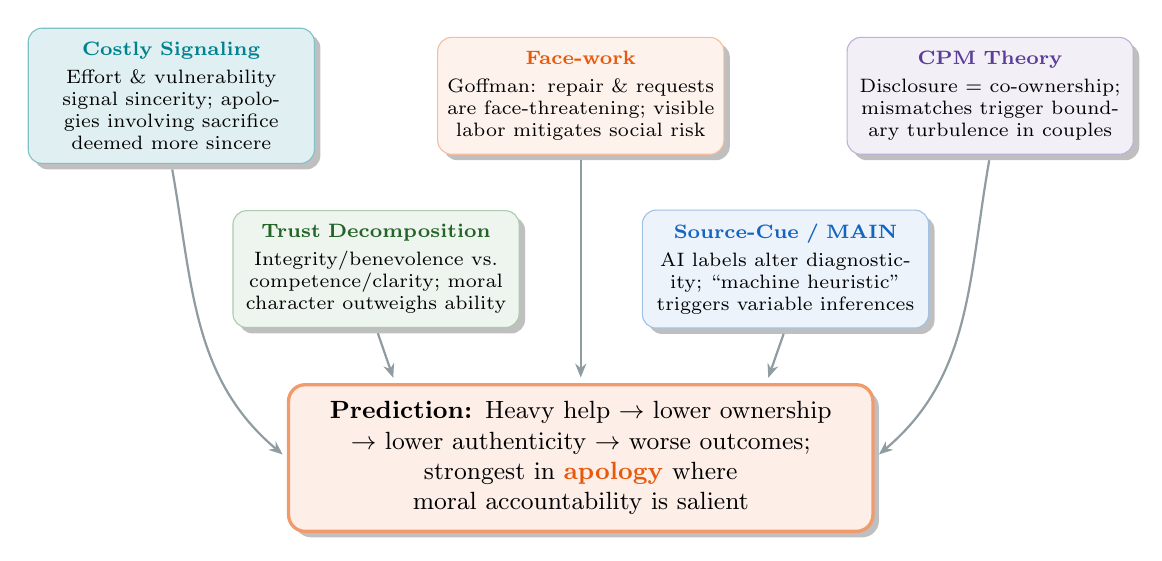
\begin{tikzpicture}[
  node distance=0.6cm and 1.3cm,
  theory/.style={rounded corners=5pt, minimum height=1.2cm, text width=3.4cm,
    align=center, font=\scriptsize, inner ysep=5pt, drop shadow},
  arr/.style={-{Stealth[length=5pt,width=4pt]}, line width=0.8pt,
    chiGray!60, shorten >=2pt, shorten <=2pt}]

  % Top row — three theory nodes
  \node[theory, fill=chiTeal!12, draw=chiTeal!50] (cst) at (-5.2,2.2)
    {\textcolor{chiTeal}{\textbf{Costly Signaling}}\\[2pt]
     Effort \& vulnerability signal sincerity; apologies involving sacrifice deemed more sincere};

  \node[theory, fill=chiAccent!8, draw=chiAccent!40] (face) at (0,2.2)
    {\textcolor{chiAccent}{\textbf{Face-work}}\\[2pt]
     Goffman: repair \& requests are face-threatening; visible labor mitigates social risk};

  \node[theory, fill=chiPurple!8, draw=chiPurple!40] (cpm) at (5.2,2.2)
    {\textcolor{chiPurple}{\textbf{CPM Theory}}\\[2pt]
     Disclosure = co-ownership; mismatches trigger boundary turbulence in couples};

  % Middle row — two theory nodes
  \node[theory, fill=chiGreen!8, draw=chiGreen!40] (trust) at (-2.6,0)
    {\textcolor{chiGreen!80!black}{\textbf{Trust Decomposition}}\\[2pt]
     Integrity/benevolence vs.\ competence/clarity; moral character outweighs ability};

  \node[theory, fill=chiBlue!8, draw=chiBlue!40] (source) at (2.6,0)
    {\textcolor{chiBlue}{\textbf{Source-Cue / MAIN}}\\[2pt]
     AI labels alter diagnosticity; ``machine heuristic'' triggers variable inferences};

  % Central prediction node
  \node[rounded corners=6pt, fill=chiAccent!10, draw=chiAccent!60, line width=1.2pt,
    text width=7cm, align=center, font=\small, inner sep=6pt, drop shadow] (pred) at (0,-2.4)
    {\textbf{Prediction:} Heavy help $\to$ lower ownership\\
     $\to$ lower authenticity $\to$ worse outcomes;\\
     strongest in \emphmark{apology} where\\
     moral accountability is salient};

  % Arrows — top row to prediction
  \draw[arr] (cst.south)   to[out=-80, in=140]  (pred.west);
  \draw[arr] (face.south)   --                    (pred.north);
  \draw[arr] (cpm.south)   to[out=-100,in=40]   (pred.east);

  % Arrows — middle row to prediction (gentle short curves, enter from upper sides)
  \draw[arr] (trust.south)  --  (pred.158);
  \draw[arr] (source.south) --   (pred.22);
\end{tikzpicture}
\end{center}
\end{frame}
% ============================================================

\begin{frame}{Two Scenarios, Two Levels of Help}
\begin{columns}[T]
\scriptsize
\begin{column}{0.47\textwidth}
  \begin{keybox}[\faExclamationTriangle~~ Apology / Repair]
    \begin{itemize}\setlength\itemsep{2pt}
      \item High moral stakes, face-threatening
      \item Demands vulnerability \& personal labor
      \item Receivers judge \emphmark{integrity} and sincerity
      \item Costly signals (effort, time) enhance forgiveness
      \item \textit{E.g., apologizing for sharing private info}
    \end{itemize}
  \end{keybox}
\end{column}
\begin{column}{0.47\textwidth}
  \begin{keybox}[\faHandPaper~~ Boundary Request]
    \begin{itemize}\setlength\itemsep{2pt}
      \item Moderate stakes, instrumentally oriented
      \item Clarity \& tact matter most
      \item Receivers judge \emphmark{competence} and reasonableness
      \item Risk: demand/withdraw dynamics, defensiveness
      \item \textit{E.g., asking partner to reduce phone use at dinner}
    \end{itemize}
  \end{keybox}
\end{column}
\end{columns}
\begin{center}
\begin{tikzpicture}[
  lvl/.style={rounded corners=4pt, minimum height=0.9cm, text width=5.3cm,
    align=center, font=\small, drop shadow}]
  \node[lvl, fill=chiGreen!10, draw=chiGreen!40] (tone) at (-4.2,0)
    {\textcolor{chiGreen}{\textbf{Tone Rewrite}} (Light Help)\\
    \footnotesize Line-level suggestions on human draft\\
    \footnotesize Content-adding blocked; human = semantic anchor};
  \node[lvl, fill=chiRed!7, draw=chiRed!30] (full) at (4.2,0)
    {\textcolor{chiRed}{\textbf{Full Draft}} (Heavy Help)\\
    \footnotesize AI generates from 2--3 bullets\\
    \footnotesize Sender must make $\geq$1 substantive edit};
  \node[font=\Large, text=chiGray] at (0,0) {\faArrowsAltH};
\end{tikzpicture}
\end{center}
\end{frame}

% ============================================================

\begin{frame}{Gaps in Prior Work}
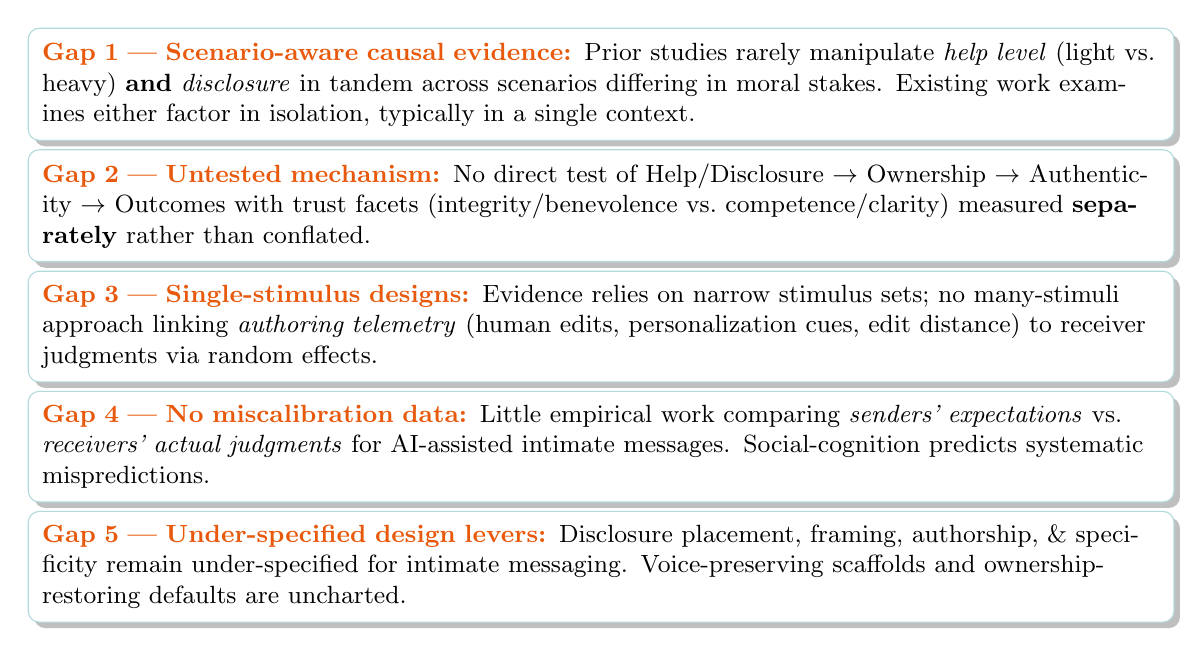
\begin{tikzpicture}[
  gap/.style={rounded corners=4pt, fill=white, draw=chiTeal!30,
    text width=14.2cm, minimum height=0.78cm, align=left, font=\small,
    inner xsep=5pt, inner ysep=5pt, drop shadow}]

  \node[gap] (g1) at (0,0) {
    \textcolor{chiAccent}{\textbf{Gap 1 --- Scenario-aware causal evidence:}} Prior studies rarely manipulate \emph{help level} (light vs.\ heavy) \textbf{and} \emph{disclosure} in tandem across scenarios differing in moral stakes. Existing work examines either factor in isolation, typically in a single context.};
  \node[gap, below=3pt of g1] (g2) {
    \textcolor{chiAccent}{\textbf{Gap 2 --- Untested mechanism:}} No direct test of Help/Disclosure $\to$ Ownership $\to$ Authenticity $\to$ Outcomes with trust facets (integrity/benevolence vs.\ competence/clarity) measured \textbf{separately} rather than conflated.};
  \node[gap, below=3pt of g2] (g3) {
    \textcolor{chiAccent}{\textbf{Gap 3 --- Single-stimulus designs:}} Evidence relies on narrow stimulus sets; no many-stimuli approach linking \emph{authoring telemetry} (human edits, personalization cues, edit distance) to receiver judgments via random effects.};
  \node[gap, below=3pt of g3] (g4) {
    \textcolor{chiAccent}{\textbf{Gap 4 --- No miscalibration data:}} Little empirical work comparing \emph{senders' expectations} vs.\ \emph{receivers' actual judgments} for AI-assisted intimate messages. Social-cognition predicts systematic mispredictions.};
  \node[gap, below=3pt of g4] (g5) {
    \textcolor{chiAccent}{\textbf{Gap 5 --- Under-specified design levers:}} Disclosure placement, framing, authorship, \& specificity remain under-specified for intimate messaging. Voice-preserving scaffolds and ownership-restoring defaults are uncharted.};
\end{tikzpicture}
\end{frame}

% ============================================================

\begin{frame}{Research Questions}
\sideAccent
\vspace{6pt}
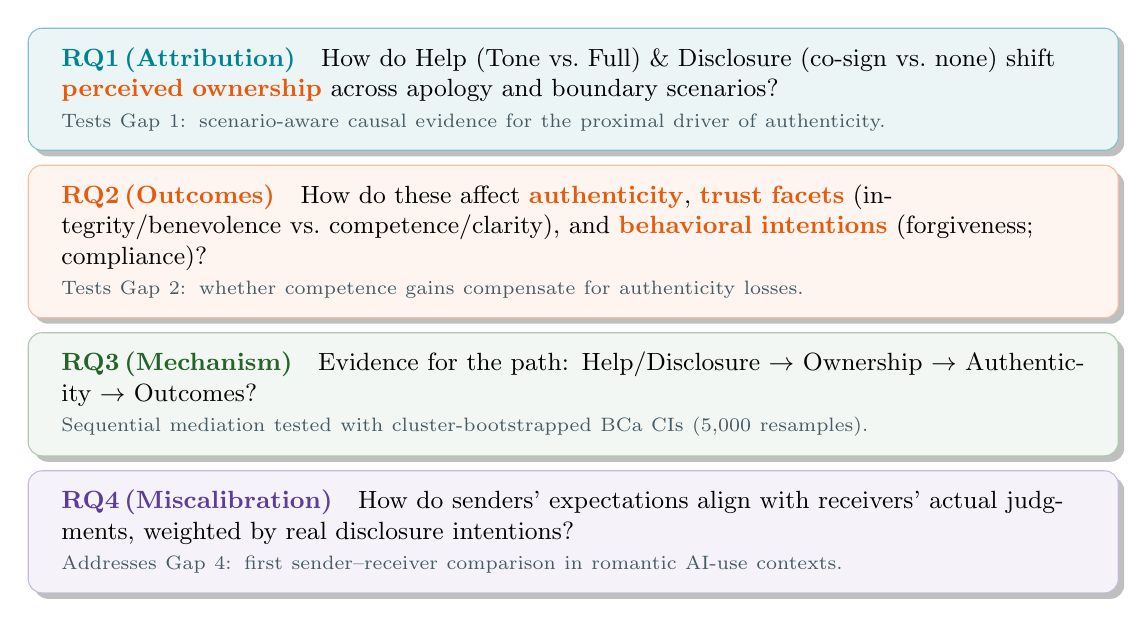
\begin{tikzpicture}[
  rq/.style={rounded corners=5pt, text width=13cm, align=left, font=\small,
    inner xsep=12pt, inner ysep=7pt,
    drop shadow}]

  \node[rq, fill=chiTeal!8, draw=chiTeal!50] (r1) at (0,0) {
    \textcolor{chiTeal}{\textbf{RQ1\,(Attribution)}} ~~How do Help (Tone vs.\ Full) \& Disclosure (co-sign vs.\ none) shift
    \emphmark{perceived ownership} across apology and boundary scenarios?\\
    {\scriptsize\textcolor{chiGray}{Tests Gap 1: scenario-aware causal evidence for the proximal driver of authenticity.}}};

  \node[rq, fill=chiAccent!6, draw=chiAccent!40, below=5pt of r1] (r2) {
    \textcolor{chiAccent}{\textbf{RQ2\,(Outcomes)}} ~~How do these affect
    \emphmark{authenticity}, \emphmark{trust facets} (integrity/benevolence vs.\ competence/clarity), and \emphmark{behavioral intentions} (forgiveness; compliance)?\\
    {\scriptsize\textcolor{chiGray}{Tests Gap 2: whether competence gains compensate for authenticity losses.}}};

  \node[rq, fill=chiGreen!6, draw=chiGreen!40, below=5pt of r2] (r3) {
    \textcolor{chiGreen!80!black}{\textbf{RQ3\,(Mechanism)}} ~~Evidence for the path:
    Help/Disclosure $\to$ Ownership $\to$ Authenticity $\to$ Outcomes?\\
    {\scriptsize\textcolor{chiGray}{Sequential mediation tested with cluster-bootstrapped BCa CIs (5{,}000 resamples).}}};

  \node[rq, fill=chiPurple!6, draw=chiPurple!35, below=5pt of r3] (r4) {
    \textcolor{chiPurple}{\textbf{RQ4\,(Miscalibration)}} ~~How do senders' expectations
    align with receivers' actual judgments, weighted by real disclosure intentions?\\
    {\scriptsize\textcolor{chiGray}{Addresses Gap 4: first sender--receiver comparison in romantic AI-use contexts.}}};
\end{tikzpicture}
\end{frame}

% ============================================================
%  SECTION: STUDY 1
% ============================================================
{
\setbeamertemplate{footline}{}
\begin{frame}[plain,noframenumbering]
\begin{tikzpicture}[remember picture, overlay]
  \fill[chiTeal] (current page.north west) rectangle
    ([yshift=-3.5cm]current page.north east);
  \mosaicCorner{-6}{1.5}{1.5}
  \mosaicCorner{5.5}{1.0}{1.2}
  \node[anchor=west, text=white, font=\huge\bfseries]
    at ([xshift=16mm, yshift=-1.75cm]current page.north west) {2};
  \node[anchor=west, text=white, font=\Large]
    at ([xshift=28mm, yshift=-1.75cm]current page.north west)
    {Study 1: Sender-Side Generative Writing};
  \draw[chiAccent, line width=2pt]
    ([xshift=16mm, yshift=-2.8cm]current page.north west) --
    ([xshift=70mm, yshift=-2.8cm]current page.north west);
  \node[anchor=north west, text=chiGray, font=\small\itshape, text width=12cm]
    at ([xshift=16mm, yshift=-4.2cm]current page.north west)
    {How do romantic partners actually use AI assistance to compose sensitive messages?};
  % Sample size badge
  \node[rounded corners=3pt, fill=chiAccent, text=white, font=\small\bfseries,
    inner xsep=10pt, inner ysep=4pt]
    at ([xshift=-25mm, yshift=-1.75cm]current page.north east) {$N{=}152$};
\end{tikzpicture}
\end{frame}
}

% ============================================================

\begin{frame}{Study 1 --- Design Overview}
\begin{center}
  \includegraphics[width=0.8\linewidth]{assets/study1.pdf}
\end{center}
\vspace{-4pt}
\begin{findingbox}
\scriptsize
\textbf{Flow:} Consent $\to$ eligibility screening (relationship $\geq$6\,mo; English fluency; keyboard required) $\to$ 1:1 randomization to Help Level $\to$ both scenarios (counterbalanced AB/BA) $\to$ post-writing scales + disclosure intentions $\to$ curation of 40 stimuli for Study~2. Sessions: $\sim$18--22 min.
\end{findingbox}
\end{frame}

% ============================================================

\begin{frame}{Study 1 --- Key Design Details}
\begin{columns}[T]
\scriptsize
\begin{column}{0.5\textwidth}
  \begin{keybox}[\faUsers~~ Participants \& Demographics]
    \begin{itemize}\setlength\itemsep{1pt}
      \item $N{=}152$ adults (from 170 consented; 18 excluded)
      \item Relationships $\geq$6\,months
      \item Recruited from Malaysia (3 university pools + social media)
      \item Mean age \textbf{31.4} (SD 6.8)
      \item Gender: 51.3\% women, 46.7\% men, 2.0\% non-binary
      \item Median relationship: 3.2\,yr [IQR 1.5, 6.0]
      \item 62.5\% cohabiting
      \item Randomized 1:1 to Tone ($n{=}76$) vs.\ Full ($n{=}76$)
      \item Both scenarios within-subjects (counterbalanced)
      \item Compensation: MYR 18 ($\sim$\$4 USD)
    \end{itemize}
  \end{keybox}
\end{column}
\begin{column}{0.5\textwidth}
  \begin{keybox}[\faClipboardList~~ Measures \& Telemetry]
    \begin{itemize}\setlength\itemsep{1pt}
      \item Felt Ownership ($\alpha{=}.87$; 3 items)
      \item Anticipated Authenticity ($\alpha{=}.90$; 3 items)
      \item Anticipated Forgiveness ($\alpha{=}.86$; Apology)
      \item Anticipated Compliance ($\alpha{=}.84$; Boundary)
      \item All 7-point Likert scales
    \end{itemize}
    \vspace{1pt}
    \textbf{Behavioral telemetry:}
    \begin{itemize}\setlength\itemsep{1pt}
      \item Edit distance (normalized Levenshtein)
      \item HCR (human-attributable chars / total)
      \item Time-on-task, assistant calls
      \item Accept/reject rate (Tone); substantive edits (Full)
      \item Idiosyncrasy cue counts (2 blind raters; $\kappa{=}.87$, ICC${=}.91$)
      \item Disclosure intention (binary + open-ended rationale)
    \end{itemize}
  \end{keybox}
\end{column}
\end{columns}
\vspace{-1pt}
\begin{center}
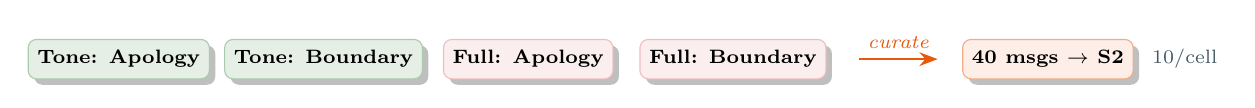
\begin{tikzpicture}[
  cell/.style={rounded corners=3pt, minimum height=0.5cm, minimum width=2cm,
    align=center, font=\scriptsize\bfseries,
    drop shadow}]
  \node[cell, fill=chiGreen!12, draw=chiGreen!40] at (-5.2,0) {Tone: Apology};
  \node[cell, fill=chiGreen!12, draw=chiGreen!40] at (-2.6,0) {Tone: Boundary};
  \node[cell, fill=chiRed!8, draw=chiRed!30] at (0,0) {Full: Apology};
  \node[cell, fill=chiRed!8, draw=chiRed!30] at (2.6,0) {Full: Boundary};
  \draw[-{Stealth}, chiAccent, thick] (4.2,0) -- node[above, font=\scriptsize\itshape] {curate} (5.2,0);
  \node[cell, fill=chiAccent!10, draw=chiAccent!50] at (6.6,0) {40 msgs $\to$ S2};
  \node[font=\scriptsize, text=chiGray, anchor=west] at (7.8,0) {10/cell};
\end{tikzpicture}
\end{center}
\end{frame}

% ============================================================

\begin{frame}{Study 1 --- Results: Ownership \& Anticipated Reactions}
\vspace{-4pt}
\begin{center}
  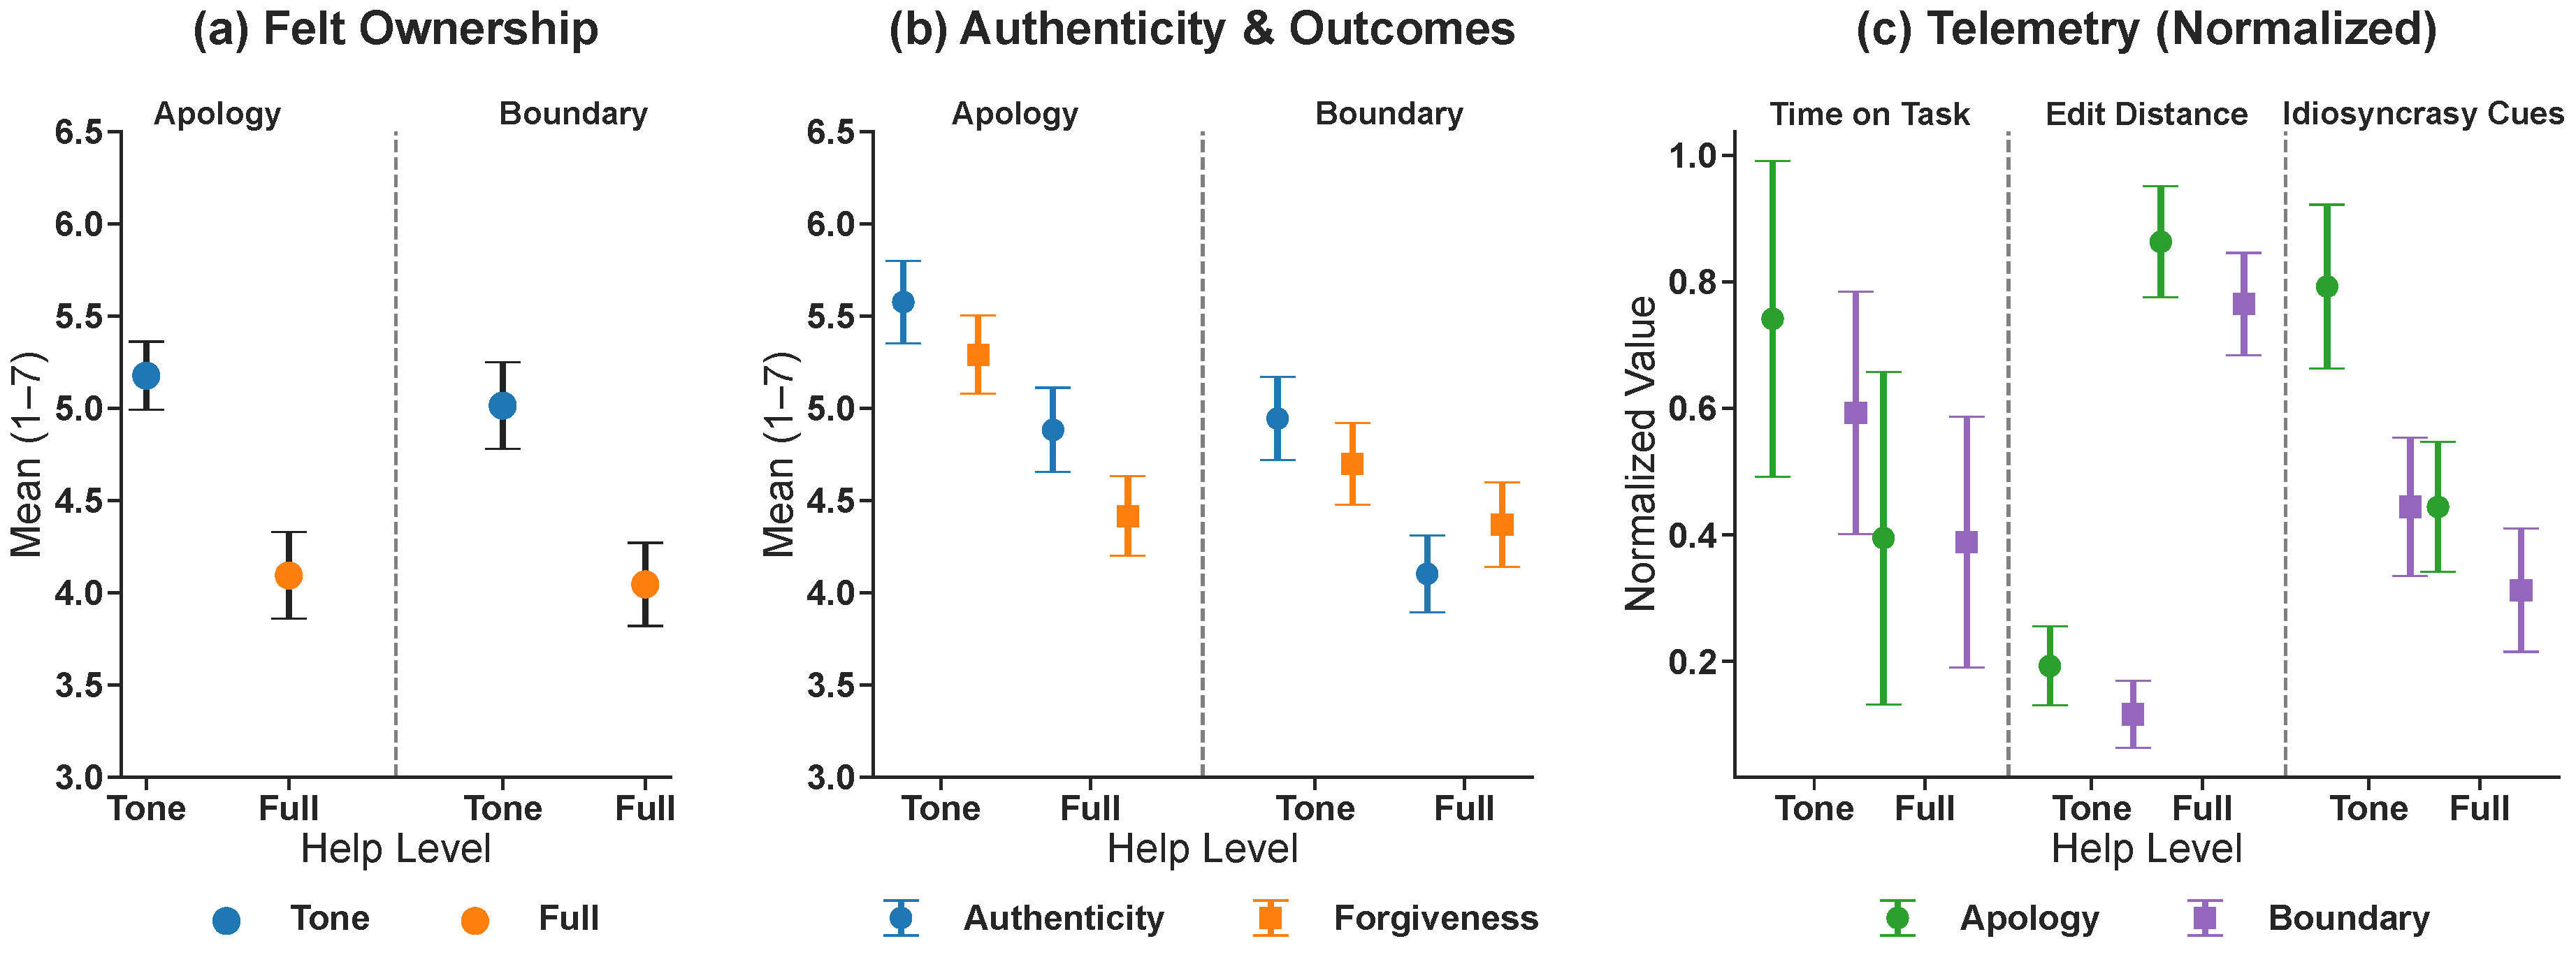
\includegraphics[width=0.84\linewidth]{assets/s1_results.pdf}
\end{center}
\vspace{-6pt}
\begin{columns}[T]
\begin{column}{0.48\textwidth}
\begin{findingbox}
\scriptsize
\textbf{Felt Ownership (LME):}\\
Full vs.\ Tone: $\beta{=}{-}0.78$, CI $[-0.98,{-}0.58]$, $t{=}{-}7.94$, $p{<}.001$\\
Boundary vs.\ Apology: $\beta{=}{-}0.32$, CI $[-0.47,{-}0.17]$, $p{<}.001$\\
Help$\times$Scenario: $\beta{=}{+}0.14$, CI $[-0.06,0.34]$, $p{=}.179$ (n.s.)
\end{findingbox}
\end{column}
\begin{column}{0.48\textwidth}
\begin{findingbox}
\scriptsize
\textbf{Anticipated Authenticity (LME):}\\
Full vs.\ Tone: $\beta{=}{-}0.65$, CI $[-0.83,{-}0.47]$, $t{=}{-}6.84$, $p{<}.001$\\
Apology help gap: $\Delta M{=}0.90$, CI $[0.62,1.18]$\\
Boundary help gap: $\Delta M{=}0.47$, CI $[0.22,0.72]$
\end{findingbox}
\end{column}
\end{columns}
\end{frame}

% ============================================================

\begin{frame}{Study 1 --- Telemetry \& Disclosure Intentions}
\vspace{1pt}
\begin{columns}[T]
\begin{column}{0.48\textwidth}
  \scriptsize
  \renewcommand{\arraystretch}{1.15}
  \begin{center}
  \begin{tabular}{@{}l cc cc@{}}
    \toprule
    & \multicolumn{2}{c}{\textbf{Apology}} & \multicolumn{2}{c}{\textbf{Boundary}}\\
    \cmidrule(lr){2-3}\cmidrule(lr){4-5}
    & \textbf{Tone} & \textbf{Full} & \textbf{Tone} & \textbf{Full}\\
    \midrule
    Time (sec) & 341 & 314 & 327 & 299\\
    Edit dist. & .19 & \textcolor{chiRed}{\textbf{.44}} & .17 & \textcolor{chiRed}{\textbf{.39}}\\
    HCR & \textcolor{chiGreen}{\textbf{.86}} & .60 & \textcolor{chiGreen}{\textbf{.84}} & .58\\
    Idio.\ cues & 1.9 & 1.5 & 1.3 & 1.0\\
    Ownership & \textcolor{chiGreen}{\textbf{5.3}} & 4.2 & 4.9 & \textcolor{chiRed}{4.1}\\
    Ant.\ Auth. & 5.6 & 4.7 & 4.9 & 4.4\\
    \bottomrule
  \end{tabular}
  \end{center}
  \vspace{3pt}
  {\scriptsize\textcolor{chiGray}{Edit distance: $\beta{=}{+}0.24$, CI $[0.20,0.28]$, $p{<}.001$.\\
   Idio.\ cues: IRR${}=0.78$, CI $[0.71,0.86]$, $p{<}.001$ (Full vs.\ Tone).\\
   HCR = Human Contribution Ratio.}}
\end{column}
\begin{column}{0.48\textwidth}
  \begin{alertbox}[\faCommentDots~~ Disclosure Intentions]
  \scriptsize
  \begin{tabular}{@{}lcc@{}}
    & \textbf{Apology} & \textbf{Boundary}\\
    \midrule
    Would disclose & \textbf{56.6\%} & 28.3\%\\
    {\scriptsize 95\% CI} & {\scriptsize [48.5, 64.3]} & {\scriptsize [21.4, 36.4]}\\
    \midrule
    Tone & 58\% & 34\%\\
    Full & 54\% & 22\%\\
  \end{tabular}
  \vspace{3pt}

  {\scriptsize OR Apology vs.\ Boundary: \textbf{3.29}, CI $[2.08,5.20]$, $p{<}.001$\\
  OR Tone vs.\ Full: \textbf{1.39}, CI $[1.02,1.89]$, $p{=}.036$}
  \vspace{4pt}

  \textcolor{chiGreen}{\faCheckCircle}~\textbf{Top ``yes'':} integrity/transparency (44\%), avoid misunderstanding (26\%), care-based (18\%)\\[2pt]
  \textcolor{chiRed}{\faTimesCircle}~\textbf{Top ``no'':} stigma (38\%), ``still my words'' (32\%), conflict risk (20\%)
  \end{alertbox}
\end{column}
\end{columns}
\end{frame}

% ============================================================

\begin{frame}{Study 1 --- Self-Report Details by Condition}
\sideAccent
\vspace{3pt}
\small
\renewcommand{\arraystretch}{1.2}
\begin{center}
\begin{tabular}{@{}l cccc@{}}
  \toprule
  & \multicolumn{2}{c}{\textbf{Apology}} & \multicolumn{2}{c}{\textbf{Boundary}}\\
  \cmidrule(lr){2-3}\cmidrule(lr){4-5}
  \textbf{Construct} & \textbf{Tone} & \textbf{Full} & \textbf{Tone} & \textbf{Full}\\
  \midrule
  Felt Ownership & 5.3 (1.1) & 4.2 (1.2) & 4.9 (1.1) & 4.1 (1.2)\\
  Ant.\ Authenticity & 5.6 (1.0) & 4.7 (1.1) & 4.9 (1.1) & 4.4 (1.1)\\
  Ant.\ Forgiveness & 5.2 (1.2) & 4.6 (1.2) & --- & ---\\
  Ant.\ Compliance & --- & --- & 4.8 (1.2) & 4.5 (1.1)\\
  \bottomrule
\end{tabular}
\end{center}

\vspace{4pt}
\begin{columns}[T]
\begin{column}{0.48\textwidth}
\begin{findingbox}
\small
\textbf{Apology:} Full $\to$ lower Anticipated Forgiveness, $\Delta M{=}0.62$, CI $[0.31,0.93]$, $p{<}.001$. Manipulation check confirmed Help separation: perceived AI contribution $5.9$ vs.\ $3.1$, $d{=}2.15$.
\end{findingbox}
\end{column}
\begin{column}{0.48\textwidth}
\begin{findingbox}
\small
\textbf{Boundary:} Smaller Help effect on Compliance, $\Delta M{=}0.30$, CI $[0.04,0.56]$, $p{=}.024$. Naturalness high \& comparable across Help (Tone $M{=}5.3$, Full $M{=}5.1$, $p{=}.217$).
\end{findingbox}
\end{column}
\end{columns}
\end{frame}

% ============================================================
%  SECTION: STUDY 2
% ============================================================
{
\setbeamertemplate{footline}{}
\begin{frame}[plain,noframenumbering]
\begin{tikzpicture}[remember picture, overlay]
  \fill[chiTeal] (current page.north west) rectangle
    ([yshift=-3.5cm]current page.north east);
  \mosaicCorner{-6}{1.5}{1.5}
  \mosaicCorner{5.5}{1.0}{1.2}
  \node[anchor=west, text=white, font=\huge\bfseries]
    at ([xshift=16mm, yshift=-1.75cm]current page.north west) {3};
  \node[anchor=west, text=white, font=\Large]
    at ([xshift=28mm, yshift=-1.75cm]current page.north west)
    {Study 2: Receiver-Side Evaluation};
  \draw[chiAccent, line width=2pt]
    ([xshift=16mm, yshift=-2.8cm]current page.north west) --
    ([xshift=70mm, yshift=-2.8cm]current page.north west);
  \node[anchor=north west, text=chiGray, font=\small\itshape, text width=12cm]
    at ([xshift=16mm, yshift=-4.2cm]current page.north west)
    {How do receivers judge AI-assisted romantic messages under controlled disclosure?};
  \node[rounded corners=3pt, fill=chiAccent, text=white, font=\small\bfseries,
    inner xsep=10pt, inner ysep=4pt]
    at ([xshift=-25mm, yshift=-1.75cm]current page.north east) {$N{=}704$};
\end{tikzpicture}
\end{frame}
}

% ============================================================

\begin{frame}{Study 2 --- Design Overview}
\vspace{-4pt}
\begin{center}
  \includegraphics[width=0.75\linewidth]{assets/study2.pdf}
\end{center}
\vspace{-5pt}
\begin{findingbox}
\scriptsize
\textbf{Panel A:} $2{\times}2$ between-subjects (Help $\times$ Disclosure), $n{=}176$/cell. \textbf{Panel B:} Each reads 1 Apology + 1 Boundary (within-subj, counterbalanced), reading-time gate $\geq$20\,s/100 words. \textbf{Panel C:} Stimuli from S1 curated pool (40 messages; 10/cell, $\sim$17.6 views each). Session: 10--14\,min.
\end{findingbox}
\end{frame}

% ============================================================

\begin{frame}{Study 2 --- Design Details}
\vspace{1pt}
\begin{columns}[T]
\scriptsize
\begin{column}{0.47\textwidth}
  \begin{keybox}[\faThLarge~~ 2$\times$2 Between-Subjects Design]
    \centering
    \scriptsize
    \renewcommand{\arraystretch}{1.4}
    \begin{tabular}{@{}l|>{\centering\arraybackslash}p{1.6cm}>{\centering\arraybackslash}p{1.6cm}@{}}
      & \textbf{No Disc.} & \textbf{Co-sign}\\
      \hline
      \textbf{Tone} & $n{=}176$ & $n{=}176$\\
      \textbf{Full} & $n{=}176$ & $n{=}176$\\
    \end{tabular}
    \vspace{4pt}

    \footnotesize Each reads 1 Apology + 1 Boundary\\ (within-subjects, counterbalanced)\\[3pt]
    {\scriptsize Powered for $d{\approx}0.20$ with BH-FDR control ($\geq$80\% power).\\
    812 consented $\to$ 704 valid after QC. No S1 overlap.\\
    Co-sign noticed: 84.1\% (miss rate 15.9\%).}
  \end{keybox}
\end{column}
\begin{column}{0.47\textwidth}
  \begin{keybox}[\faClipboardCheck~~ Receiver Measures]
    \begin{itemize}\setlength\itemsep{2pt}
      \item[\faUserCheck] Effort/Ownership ($\alpha{=}.87$--.89; 3 items; 1-factor CFA confirmed)
      \item[\faHeart] Authenticity ($\alpha{=}.90$--.91; 3 items)
      \item[\faLock] Trust: Integrity/Benev.\ ($\alpha{=}.86$--.88; 3 items)
      \item[\faStar] Trust: Competence/Clarity ($\alpha{=}.85$--.86; 3 items)
      \item[\faHandshake] Forgiveness ($\alpha{=}.88$) / Compliance ($\alpha{=}.85$)
      \item[\faCog] Covariates: AI attitude ($\alpha{=}.82$), relationship length
    \end{itemize}
    {\scriptsize LME with crossed random intercepts for participant \& stimulus; effect-coded ($\pm 0.5$). BH-FDR within DV$\times$Scenario.}
  \end{keybox}
\end{column}
\end{columns}
\vspace{4pt}
\begin{center}
  
\begin{tikzpicture}[font=\scriptsize]
    \node[rounded corners=4pt, fill=chiTeal!8, draw=chiTeal!40,
      inner sep=7pt, text width=12cm, align=center] {
      \textbf{Co-sign disclosure:} \emph{``I used an AI tool to help me phrase this clearly.''}\\[2pt]
      \footnotesize Sender-voiced $\cdot$ Clarity-framed $\cdot$ Appended as final line $\cdot$ Same across scenarios $\cdot$ One point in a broader design space};
  \end{tikzpicture}
\end{center}
\end{frame}

% ============================================================

\begin{frame}{What Do These Messages Actually Look Like?}
\vspace{1pt}
\begin{columns}[T]
\scriptsize
\begin{column}{0.47\textwidth}
  \begin{examplebox}[\faPen~~ Tone Rewrite (Light Help) --- Apology]
  \footnotesize\itshape
  ``I've been thinking about what happened after [the party at Mei's place] last Saturday, and I need to say I'm sorry. I shouldn't have shared what you told me about your sister --- that was your story to tell, not mine. I know you trusted me with something personal, and I broke that trust. I want to earn it back. Can we talk about this tonight after dinner? I love you, [Bean].''
  \end{examplebox}
  \vspace{2pt}
  {\scriptsize\textcolor{chiGray}{Human draft preserved; AI only adjusted tone/phrasing. Idiosyncrasy cues: nickname, shared memory, specific time/place. HCR $\approx 0.86$.}}
\end{column}
\begin{column}{0.47\textwidth}
  \begin{examplebox}[\faRobot~~ Full Draft (Heavy Help) --- Apology]
  \footnotesize\itshape
  ``I want to sincerely apologize for sharing something you told me in confidence. I realize that what I did was a violation of your trust, and I deeply regret it. Your feelings matter to me, and I should have been more thoughtful about respecting your privacy. I am committed to being more careful in the future and to rebuilding the trust between us. I hope you can give me the chance to make things right.''
  \end{examplebox}
  \vspace{2pt}
  {\scriptsize\textcolor{chiRed}{AI-generated from bullets; sender edited lightly. Generic language, no idiosyncrasy cues, formulaic phrasing. HCR $\approx 0.60$.}}
\end{column}
\end{columns}
\vspace{4pt}
\begin{findingbox}
\scriptsize
\textbf{Key contrast:} Same apology intent, but Tone preserves ``voice'' (shared memories, nicknames, specifics) while Full produces polished but \emphmark{generic} text. Receivers detect this difference even without being told about AI use.
\end{findingbox}
\end{frame}

% ============================================================

\begin{frame}{Study 2 --- Estimated Marginal Means (EMMs)}
\sideAccent
\vspace{2pt}
\scriptsize
\renewcommand{\arraystretch}{1.15}
\begin{center}
\begin{tabular}{@{}l cccc@{}}
  \toprule
  \textbf{Variable} & \textbf{Tone/None} & \textbf{Tone/CoSign} & \textbf{Full/None} & \textbf{Full/CoSign}\\
  \midrule
  \multicolumn{5}{l}{\textit{Apology Scenario}} \\
  \midrule
  Effort/Ownership & 5.0 (1.1) & 4.9 (1.1) & 4.2 (1.2) & 4.0 (1.2)\\
  Authenticity & 5.1 (1.0) & \textcolor{chiGreen}{\textbf{5.4}} (1.0) & 4.7 (1.1) & \textcolor{chiRed}{4.6} (1.1)\\
  Trust--Integrity/Benev. & 5.1 (1.1) & 5.3 (1.0) & 4.6 (1.1) & 4.4 (1.1)\\
  Trust--Competence/Clarity & 5.0 (1.0) & 5.1 (1.0) & \textcolor{chiBlue}{\textbf{5.4}} (0.9) & \textcolor{chiBlue}{\textbf{5.5}} (0.9)\\
  Forgiveness & 4.9 (1.2) & \textcolor{chiGreen}{\textbf{5.2}} (1.1) & 4.7 (1.2) & \textcolor{chiRed}{4.6} (1.2)\\
  \midrule
  \multicolumn{5}{l}{\textit{Boundary Scenario}} \\
  \midrule
  Effort/Ownership & 4.5 (1.1) & 4.3 (1.1) & 4.1 (1.1) & 3.9 (1.1)\\
  Authenticity & 4.7 (1.1) & 4.6 (1.1) & 4.3 (1.1) & 4.2 (1.1)\\
  Trust--Integrity/Benev. & 4.7 (1.1) & 4.5 (1.1) & 4.4 (1.0) & 4.2 (1.0)\\
  Trust--Competence/Clarity & 4.9 (1.0) & 5.0 (1.0) & \textcolor{chiBlue}{\textbf{5.3}} (0.9) & \textcolor{chiBlue}{\textbf{5.4}} (0.9)\\
  Compliance & 4.6 (1.2) & 4.5 (1.2) & 4.5 (1.1) & 4.3 (1.1)\\
  \bottomrule
\end{tabular}
\end{center}
\vspace{2pt}
{\footnotesize\textcolor{chiGray}{All scales 1--7 (SD in parentheses). \textcolor{chiGreen}{\textbf{Green}} = best condition.
\textcolor{chiRed}{\textbf{Red}} = worst. \textcolor{chiBlue}{\textbf{Blue}} = competence gain that does not improve outcomes. Manip check: perceived AI contribution Full $5.7$ vs.\ Tone $3.3$, $d{=}1.82$, $p{<}.001$.}}
\end{frame}

% ============================================================

\begin{frame}{Study 2 --- Results: Authenticity \& Outcomes}
\sideAccent
\vspace{-4pt}
\begin{center}
  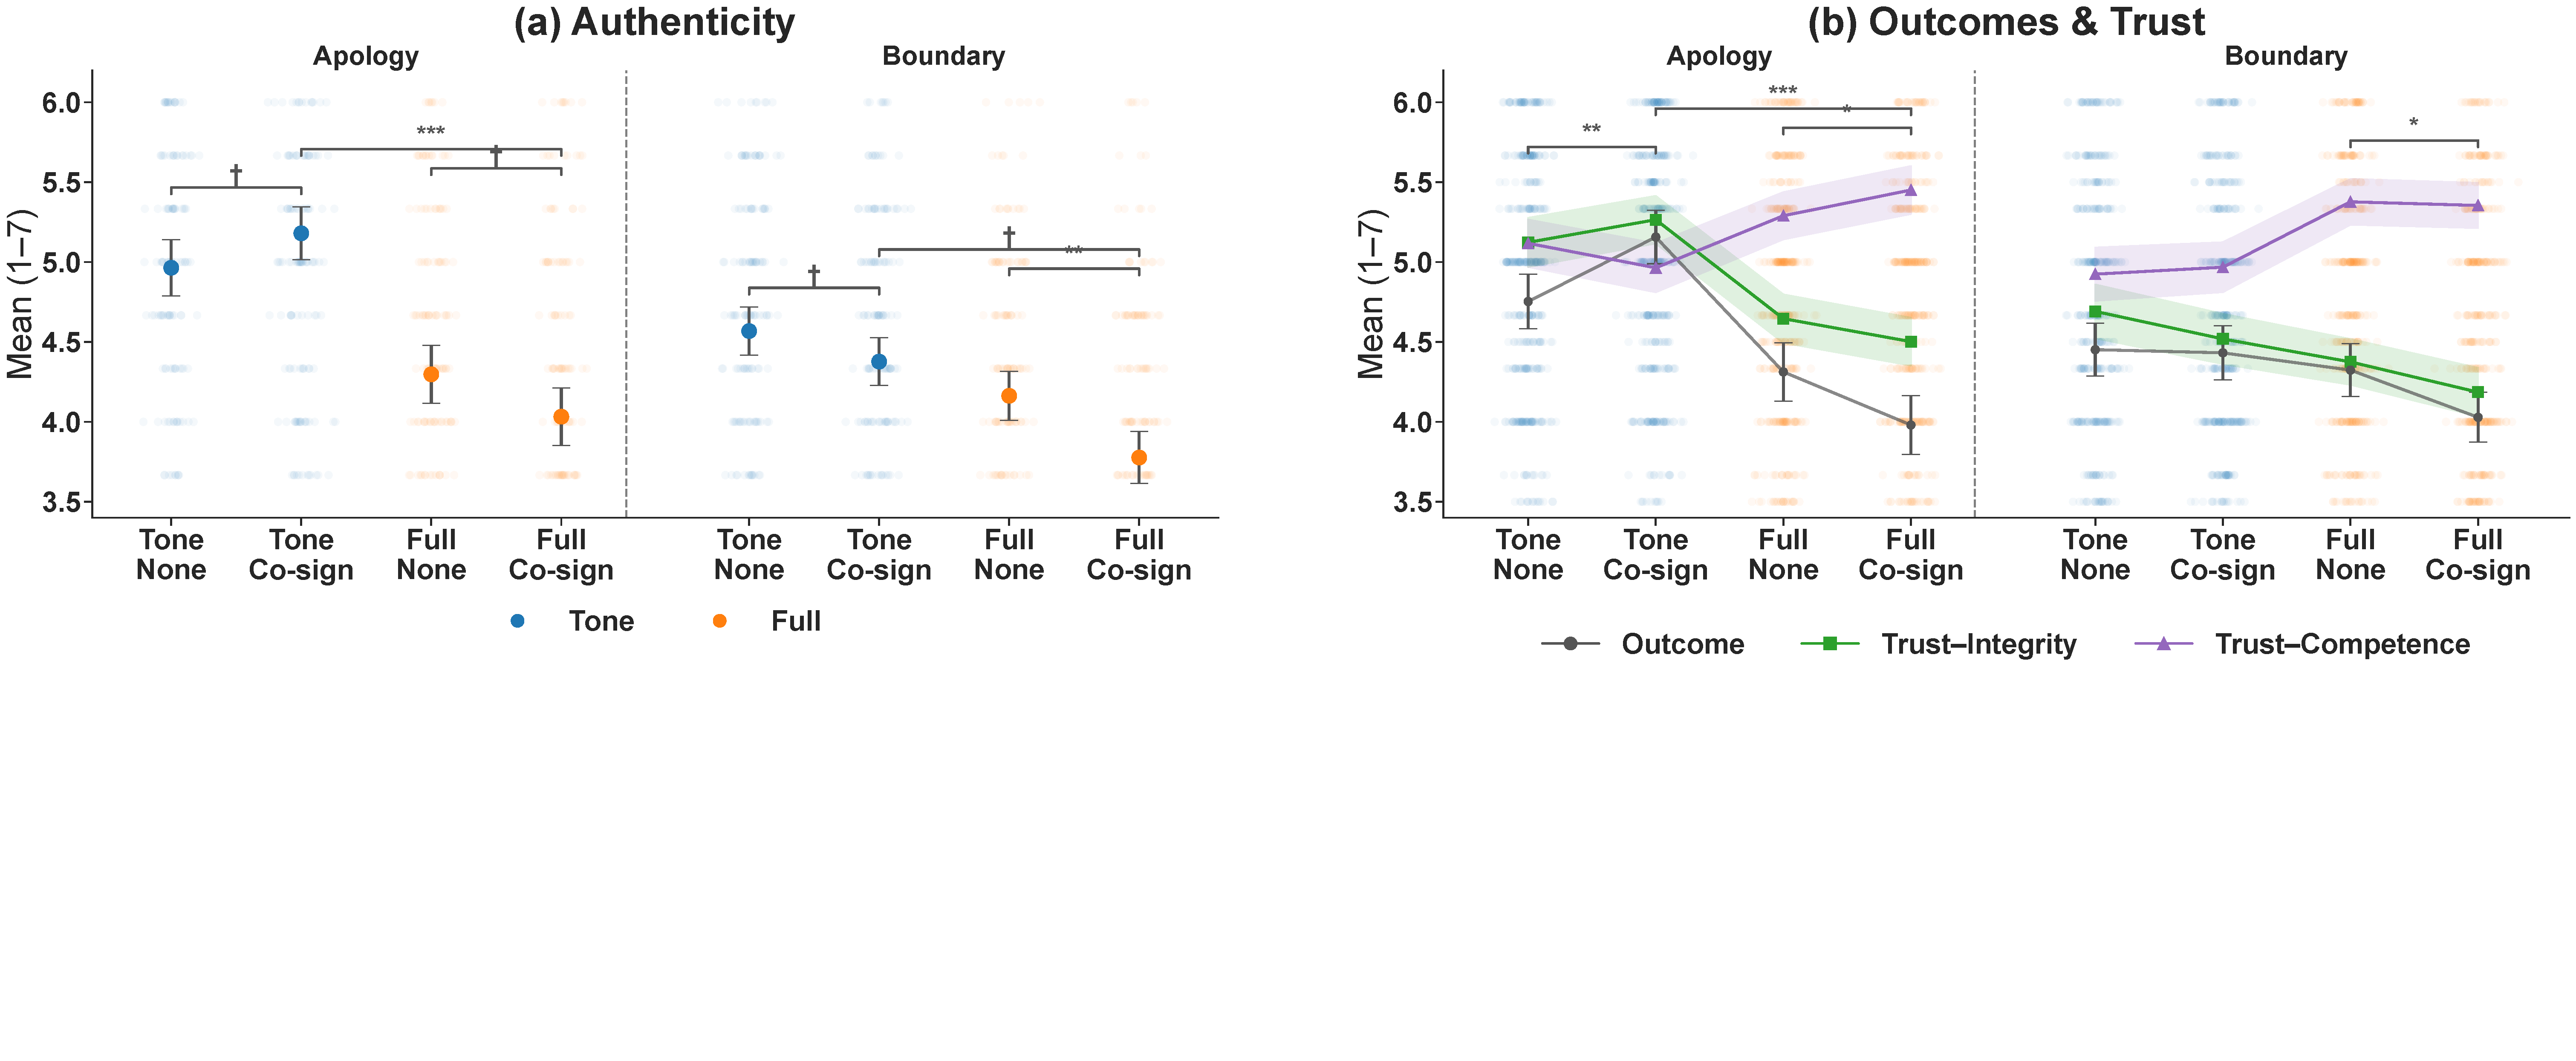
\includegraphics[width=0.84\linewidth]{assets/s2_results.pdf}
\end{center}
\vspace{-6pt}
\begin{columns}[T]
\begin{column}{0.48\textwidth}
\begin{findingbox}
\small
\textbf{Apology:} Co-signing Tone \good{raised} authenticity ($+0.30$, CI $[+.18,+.42]$, $d{=}0.28$, $p{<}.001$) \& forgiveness ($+0.28$, $d{=}0.24$, $p{=}.002$).
Co-signing Full \bad{lowered} both ($-0.11$/$-0.12$).
\end{findingbox}
\end{column}
\begin{column}{0.48\textwidth}
\begin{findingbox}
\small
\textbf{Boundary:} Co-signing had \neutral{small / marginally negative} effects. C1 Authenticity: $-0.12$, CI $[-0.23,-0.01]$, $p{=}.051$. C1 Compliance: $-0.12$, $p{=}.112$ (n.s.). Help penalty (C3) still reliable: $-0.40$, $p{<}.001$.
\end{findingbox}
\end{column}
\end{columns}
\end{frame}

% ============================================================

\begin{frame}{Study 2 --- Planned Contrasts: Apology}
\vspace{4pt}
\small
\renewcommand{\arraystretch}{1.3}
\begin{center}
\begin{tabular}{@{}p{4.4cm} p{4.6cm} p{4.2cm}@{}}
  \toprule
  \textbf{Contrast} & \textbf{Authenticity} & \textbf{Forgiveness}\\
  \midrule
  \textbf{C1:} Tone+CoSign \newline vs Tone+None
    & \textcolor{chiGreen}{\textbf{+0.30}} {\scriptsize[+.18,+.42]} \newline $d{=}0.28$, $p{<}.001$
    & \textcolor{chiGreen}{\textbf{+0.28}} {\scriptsize[+.11,+.44]} \newline $d{=}0.24$, $p{=}.002$\\[4pt]
  \textbf{C2:} Full+CoSign \newline vs Full+None
    & \textcolor{chiRed}{\textbf{--0.11}} {\scriptsize[--0.20,--0.02]} \newline $d{=}{-}0.10$, $p{=}.018$
    & \textcolor{chiRed}{\textbf{--0.12}} {\scriptsize[--0.24,0.00]} \newline $d{=}{-}0.11$, $p{=}.049$\\[4pt]
  \textbf{C3:} Full+CoSign \newline vs Tone+CoSign
    & \textcolor{chiRed}{\textbf{--0.83}} {\scriptsize[--0.98,--0.68]} \newline $d{=}{-}0.76$, $p{<}.001$
    & \textcolor{chiRed}{\textbf{--0.63}} {\scriptsize[--0.80,--0.46]} \newline $d{=}{-}0.54$, $p{<}.001$\\
  \bottomrule
\end{tabular}
\end{center}

\vspace{3pt}
\begin{findingbox}
\small
\faLightbulb~~ The \emphmark{same disclosure label} has \textbf{opposite effects} depending on help level:
integrity cue for light help vs.\ outsourcing spotlight for heavy help. C3 ($d{=}{-}0.76$ for Authenticity) is the largest effect in the study.
\end{findingbox}
\end{frame}

% ============================================================

\begin{frame}{Study 2 --- Planned Contrasts: Boundary Request}
\sideAccent
\vspace{4pt}
\small
\renewcommand{\arraystretch}{1.3}
\begin{center}
\begin{tabular}{@{}p{4.4cm} p{4.6cm} p{4.2cm}@{}}
  \toprule
  \textbf{Contrast} & \textbf{Authenticity} & \textbf{Compliance}\\
  \midrule
  \textbf{C1:} Tone+CoSign \newline vs Tone+None
    & \textcolor{chiGray}{\textbf{--0.12}} {\scriptsize[--0.23,--0.01]} \newline $d{=}{-}0.11$, $p{=}.051$
    & \textcolor{chiGray}{\textbf{--0.12}} {\scriptsize[--0.25,+0.02]} \newline $d{=}{-}0.10$, $p{=}.112$\\[4pt]
  \textbf{C2:} Full+CoSign \newline vs Full+None
    & \textcolor{chiGray}{\textbf{--0.10}} {\scriptsize[--0.21,+0.01]} \newline $d{=}{-}0.09$, $p{=}.088$
    & \textcolor{chiRed}{\textbf{--0.14}} {\scriptsize[--0.29,+0.01]} \newline $d{=}{-}0.12$, $p{=}.074$\\[4pt]
  \textbf{C3:} Full+CoSign \newline vs Tone+CoSign
    & \textcolor{chiRed}{\textbf{--0.40}} {\scriptsize[--0.56,--0.24]} \newline $d{=}{-}0.35$, $p{<}.001$
    & \textcolor{chiRed}{\textbf{--0.20}} {\scriptsize[--0.35,--0.05]} \newline $d{=}{-}0.18$, $p{=}.010$\\
  \bottomrule
\end{tabular}
\end{center}

\vspace{3pt}
\begin{findingbox}
\small
\faLightbulb~~ In \textbf{Boundary} requests, co-signing provides \emphmark{no benefit} --- effects are neutral to mildly negative. The Help penalty (C3) is reliable but smaller than in Apology ($d{=}{-}0.35$ vs.\ $-0.76$ for Authenticity). This scenario demands clarity more than moral labor; yet heavy help still hurts.
\end{findingbox}
\end{frame}

% ============================================================

\begin{frame}{Study 2 --- Trust Decomposition}
\sideAccent
\vspace{4pt}
\begin{columns}[T]
\begin{column}{0.48\textwidth}
  \begin{keybox}[\faLock~~ Integrity/Benevolence]
  \scriptsize
  \textbf{Tracks Authenticity closely:}
  \begin{itemize}\setlength\itemsep{3pt}
    \item Apology C1 (Tone co-sign benefit):\\
      $+0.22$, CI $[+0.10,+0.34]$, $p{<}.001$
    \item Apology C3 (Help penalty):\\
      $\mathbf{-0.87}$, CI $[-1.03,-0.71]$, $p{<}.001$
    \item Boundary C3:\\
      $-0.30$, CI $[-0.46,-0.14]$, $p{<}.001$
  \end{itemize}
  \vspace{3pt}
  {\scriptsize Integrity/benevolence mirrors authenticity: when perceived ownership drops, so does moral trust.}
  \end{keybox}
\end{column}
\begin{column}{0.48\textwidth}
  \begin{alertbox}[\faStar~~ Competence/Clarity]
  \scriptsize
  \textbf{Improves under Full --- but irrelevant to outcomes:}
  \begin{itemize}\setlength\itemsep{3pt}
    \item Apology C3: \textcolor{chiBlue}{\textbf{+0.39}}, CI $[+0.26,+0.52]$, $p{<}.001$
    \item Boundary C3: \textcolor{chiBlue}{\textbf{+0.41}}, CI $[+0.28,+0.54]$, $p{<}.001$
  \end{itemize}
  \vspace{3pt}
  \textbf{Partial assoc.\ with Outcomes (controlling Authenticity):}
  \begin{itemize}\setlength\itemsep{3pt}
    \item Apology: $\beta{=}+0.06$, $p{=}.138$ (n.s.)
    \item Boundary: $\beta{=}+0.10$, $p{=}.012$ (small)
  \end{itemize}
  \vspace{3pt}
  {\scriptsize \emphmark{Better-sounding $\neq$ better-received} when ownership is in doubt.}
  \end{alertbox}
\end{column}
\end{columns}
\end{frame}

% ============================================================

\begin{frame}{Study 2 --- The Competence Dissociation}
\sideAccent
\vspace{4pt}
\begin{columns}[T]
\begin{column}{0.52\textwidth}
  \begin{tikzpicture}[
    node distance=0.9cm,
    box/.style={rounded corners=4pt, minimum height=1cm, text width=3.6cm,
      align=center, font=\small,
      drop shadow}]

    \node[box, fill=chiGray!10, draw=chiGray!40] (full) at (0,3.2)
      {\textbf{Full Draft (Heavy AI)}};

    \node[box, fill=chiGreen!12, draw=chiGreen!40] (comp) at (-2.2,1.2)
      {\faStar~~Competence\\Clarity \textcolor{chiGreen}{\textbf{UP}}\\
      {\scriptsize Apo: +0.39, Bnd: +0.41}};
    \node[box, fill=chiRed!8, draw=chiRed!30] (auth) at (2.2,1.2)
      {\faHeartBroken~~Authenticity\\Integrity \textcolor{chiRed}{\textbf{DOWN}}\\
      {\scriptsize Apo: $-$0.83, Bnd: $-$0.40}};

    \node[box, fill=chiRed!10, draw=chiRed!40] (out) at (0,-0.8)
      {\faThumbsDown~~Forgiveness / Compliance \textcolor{chiRed}{\textbf{DOWN}}\\
      {\scriptsize Apo: $-$0.63, Bnd: $-$0.20}};

    \draw[-{Stealth}, thick, chiGreen!70!black] (full.south west) -- (comp.north);
    \draw[-{Stealth}, thick, chiRed!70!black] (full.south east) -- (auth.north);
    \draw[-{Stealth}, thick, chiRed, line width=2pt]
      (auth.south) -- node[right=2pt, font=\scriptsize\bfseries, text=chiRed] {drives} (out.north east);
    \draw[-{Stealth}, dashed, chiGray, thick]
      (comp.south) -- node[left=2pt, font=\scriptsize, text=chiGray] {weak} (out.north west);
  \end{tikzpicture}
\end{column}
\begin{column}{0.44\textwidth}
  \begin{alertbox}[P3: Competence $\neq$ Outcomes]
    \scriptsize
    Full help raised Competence/Clarity:
    \begin{itemize}\setlength\itemsep{2pt}
      \item Apology: $+0.39$, $p{<}.001$
      \item Boundary: $+0.41$, $p{<}.001$
    \end{itemize}
    \vspace{3pt}
    But Competence had \emphmark{weak/null} association with outcomes once Authenticity controlled:
    \begin{itemize}\setlength\itemsep{2pt}
      \item Apology: $\beta{=}+0.06$, CI $[-0.02,+0.14]$, $p{=}.138$
      \item Boundary: $\beta{=}+0.10$, CI $[+0.02,+0.18]$, $p{=}.012$
    \end{itemize}
    \vspace{3pt}
    {\scriptsize Forgiveness penalty unchanged after covariate adjustment: $\Delta{=}-0.61$ unadjusted vs.\ $-0.58$ adjusted, both $p{<}.001$.}
  \end{alertbox}
\end{column}
\end{columns}
\end{frame}

% ============================================================

\begin{frame}{Study 2 --- Sequential Mediation: Apology}
\sideAccent
\vspace{4pt}
\begin{center}
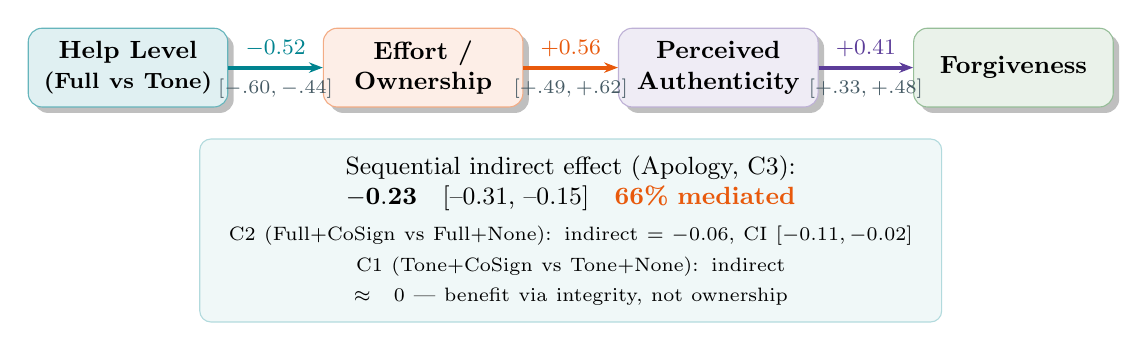
\begin{tikzpicture}[
  node distance=1.2cm,
  pathbox/.style={rounded corners=5pt, minimum height=1cm, text width=2.3cm,
    align=center, font=\small\bfseries,
    drop shadow},
  arr/.style={-{Stealth[length=5pt]}, line width=1.4pt}]

  \node[pathbox, fill=chiTeal!12, draw=chiTeal!60] (help) {Help Level\\{\footnotesize(Full vs Tone)}};
  \node[pathbox, fill=chiAccent!10, draw=chiAccent!50, right=of help] (own) {Effort /\\Ownership};
  \node[pathbox, fill=chiPurple!10, draw=chiPurple!40, right=of own] (auth) {Perceived\\Authenticity};
  \node[pathbox, fill=chiGreen!10, draw=chiGreen!50, right=of auth] (out) {Forgiveness};

  \draw[arr, chiTeal] (help) -- node[above, font=\footnotesize\bfseries, text=chiTeal] {$-0.52$} node[below, font=\scriptsize, text=chiGray] {{\scriptsize[$-.60,-.44$]}} (own);
  \draw[arr, chiAccent] (own) -- node[above, font=\footnotesize\bfseries, text=chiAccent] {$+0.56$} node[below, font=\scriptsize, text=chiGray] {{\scriptsize[$+.49,+.62$]}} (auth);
  \draw[arr, chiPurple] (auth) -- node[above, font=\footnotesize\bfseries, text=chiPurple] {$+0.41$} node[below, font=\scriptsize, text=chiGray] {{\scriptsize[$+.33,+.48$]}} (out);

  % Annotation
  \node[below=0.9cm of $(own)!0.5!(auth)$, rounded corners=4pt, fill=chiTeal!6, draw=chiTeal!30,
    inner sep=6pt, text width=9cm, align=center, font=\small]
    {Sequential indirect effect (Apology, C3):
    $\mathbf{-0.23}$ ~~[--0.31, --0.15] ~~\textcolor{chiAccent}{\textbf{66\% mediated}}\\[2pt]
    {\scriptsize C2 (Full+CoSign vs Full+None): indirect $= -0.06$, CI $[-0.11,-0.02]$}\\
    {\scriptsize C1 (Tone+CoSign vs Tone+None): indirect $\approx 0$ --- benefit via integrity, not ownership}};
\end{tikzpicture}
\end{center}

\vspace{3pt}
\begin{findingbox}
\small
\textbf{C1 mechanism:} The co-sign benefit for Tone operates via \emphmark{integrity-driven authenticity} ($+0.14$, CI $[+0.07,+0.22]$), not through ownership change. This distinguishes transparency signals from effort/authorship signals.
\end{findingbox}
\end{frame}

% ============================================================

\begin{frame}{Study 2 --- Sequential Mediation: Boundary}
\sideAccent
\vspace{4pt}
\begin{center}
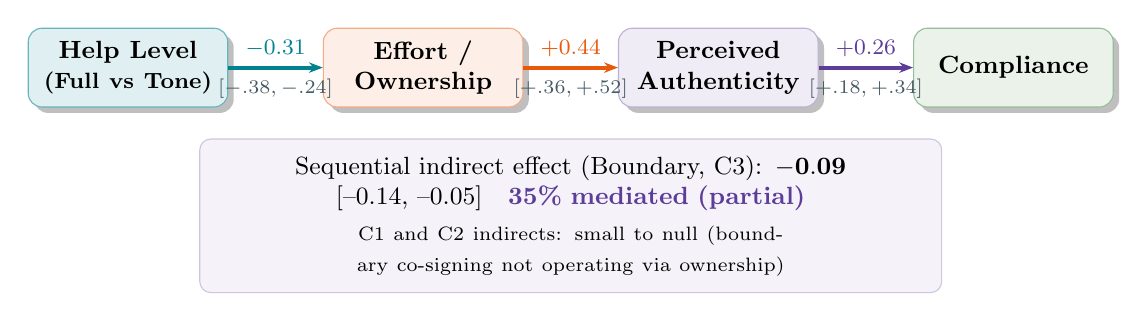
\begin{tikzpicture}[
  node distance=1.2cm,
  pathbox/.style={rounded corners=5pt, minimum height=1cm, text width=2.3cm,
    align=center, font=\small\bfseries,
    drop shadow},
  arr/.style={-{Stealth[length=5pt]}, line width=1.4pt}]

  \node[pathbox, fill=chiTeal!12, draw=chiTeal!60] (help) {Help Level\\{\footnotesize(Full vs Tone)}};
  \node[pathbox, fill=chiAccent!10, draw=chiAccent!50, right=of help] (own) {Effort /\\Ownership};
  \node[pathbox, fill=chiPurple!10, draw=chiPurple!40, right=of own] (auth) {Perceived\\Authenticity};
  \node[pathbox, fill=chiGreen!10, draw=chiGreen!50, right=of auth] (out) {Compliance};

  \draw[arr, chiTeal] (help) -- node[above, font=\footnotesize\bfseries, text=chiTeal] {$-0.31$} node[below, font=\scriptsize, text=chiGray] {{\scriptsize[$-.38,-.24$]}} (own);
  \draw[arr, chiAccent] (own) -- node[above, font=\footnotesize\bfseries, text=chiAccent] {$+0.44$} node[below, font=\scriptsize, text=chiGray] {{\scriptsize[$+.36,+.52$]}} (auth);
  \draw[arr, chiPurple] (auth) -- node[above, font=\footnotesize\bfseries, text=chiPurple] {$+0.26$} node[below, font=\scriptsize, text=chiGray] {{\scriptsize[$+.18,+.34$]}} (out);

  % Annotation
  \node[below=0.9cm of $(own)!0.5!(auth)$, rounded corners=4pt, fill=chiPurple!6, draw=chiPurple!30,
    inner sep=6pt, text width=9cm, align=center, font=\small]
    {Sequential indirect effect (Boundary, C3):
    $\mathbf{-0.09}$ ~~[--0.14, --0.05] ~~\textcolor{chiPurple}{\textbf{35\% mediated (partial)}}\\[2pt]
    {\scriptsize C1 and C2 indirects: small to null (boundary co-signing not operating via ownership)}};
\end{tikzpicture}
\end{center}

\vspace{3pt}
\begin{findingbox}
\small
\textbf{Comparison:} Apology mediation is \textbf{strong} (66\%, indirect $= -0.23$); Boundary is \textbf{partial} (35\%, indirect $= -0.09$). Path coefficients are weaker at every link for boundary requests. This confirms \emphmark{scenario sensitivity}: moral accountability amplifies the ownership mechanism.
\end{findingbox}
\end{frame}

% ============================================================
%  SECTION: INTEGRATION
% ============================================================
{
\setbeamertemplate{footline}{}
\begin{frame}[plain,noframenumbering]
\begin{tikzpicture}[remember picture, overlay]
  \fill[chiTeal] (current page.north west) rectangle
    ([yshift=-3.5cm]current page.north east);
  \mosaicCorner{-6}{1.5}{1.5}
  \mosaicCorner{5.5}{1.0}{1.2}
  \node[anchor=west, text=white, font=\huge\bfseries]
    at ([xshift=16mm, yshift=-1.75cm]current page.north west) {4};
  \node[anchor=west, text=white, font=\Large]
    at ([xshift=28mm, yshift=-1.75cm]current page.north west)
    {Cross-Study Integration};
  \draw[chiAccent, line width=2pt]
    ([xshift=16mm, yshift=-2.8cm]current page.north west) --
    ([xshift=70mm, yshift=-2.8cm]current page.north west);
  \node[anchor=north west, text=chiGray, font=\small\itshape, text width=12cm]
    at ([xshift=16mm, yshift=-4.2cm]current page.north west)
    {Linking authoring traces to receiver attributions and quantifying sender--receiver gaps};
\end{tikzpicture}
\end{frame}
}

% ============================================================

\begin{frame}{Integration --- Authoring Traces Predict Receiver Judgments}
\vspace{-6pt}
\begin{center}
  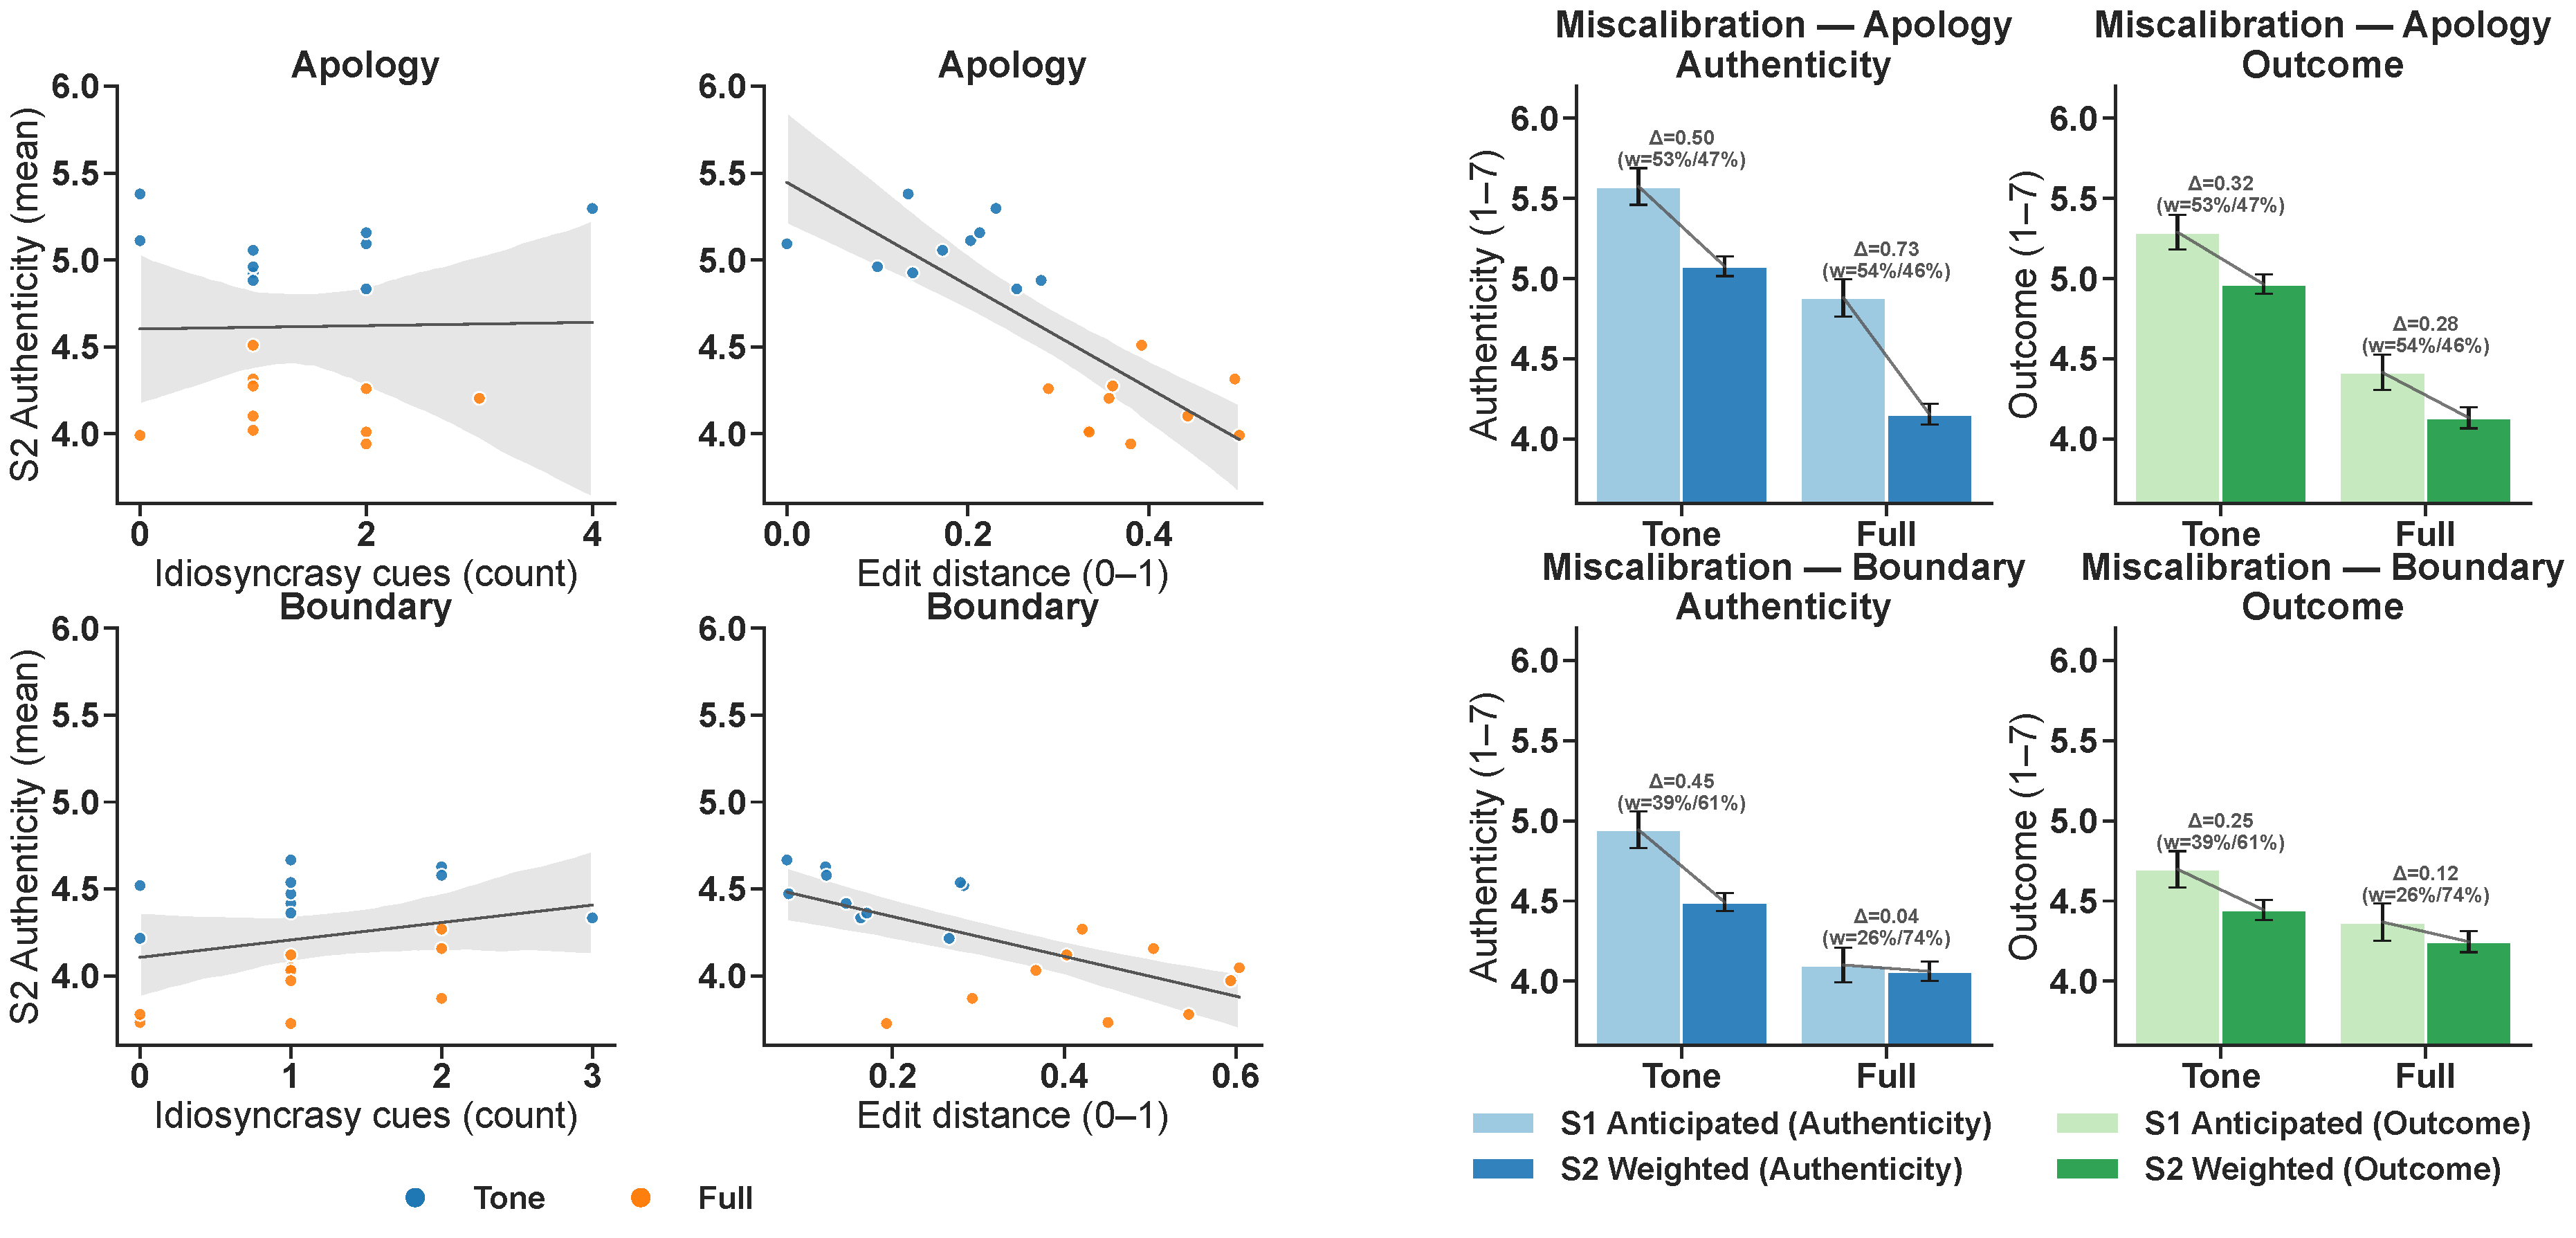
\includegraphics[width=0.78\linewidth, height=0.46\textheight, keepaspectratio]{assets/integration_combined.pdf}
\end{center}
\vspace{-5pt}
\begin{columns}[T]
\begin{column}{0.5\textwidth}
  \begin{findingbox}
    \scriptsize \good{More idiosyncrasy cues}\\
    $\to$ higher Ownership: $\beta{=}{+}0.18$, CI $[+.12,+.24]$, $p{<}.001$\\
    $\to$ higher Authenticity: $\beta{=}{+}0.16$, CI $[+.10,+.22]$, $p{<}.001$\\
    {\scriptsize Apology: $\beta{=}+0.21$; Boundary: $\beta{=}+0.14$}\\[3pt]
    \good{Higher HCR} $\to$ higher ownership, authenticity\\
    {\scriptsize S1 Felt Ownership correlates with S2 Effort/Ownership: Apology $r{=}.41$, Boundary $r{=}.28$}
  \end{findingbox}
\end{column}
\begin{column}{0.55\textwidth}
  \begin{findingbox}
    \scriptsize \bad{Greater edit distance}\\
    $\to$ lower Ownership: $\beta{=}{-}0.17$, CI $[-.25,-.09]$, $p{<}.001$\\
    $\to$ lower Authenticity: $\beta{=}{-}0.12$, CI $[-.19,-.05]$, $p{=}.001$\\[3pt]
    {\scriptsize \textbf{Scatterplots show:} each point is a unique message (40 total), colored by Help. Tone clusters at higher authenticity; Full at lower. Lines show linear best fit with 95\% CIs.}\\[3pt]
    {\scriptsize Trust--Integrity tracks Authenticity closely (Apology $\beta{=}+0.62$; Boundary $\beta{=}+0.49$).}
  \end{findingbox}
\end{column}
\end{columns}
\end{frame}

% ============================================================

\begin{frame}{Integration --- Sender--Receiver Miscalibration}
\sideAccent
\vspace{4pt}
\begin{columns}[T]
\begin{column}{0.48\textwidth}
  \scriptsize
  \renewcommand{\arraystretch}{1.25}
  \begin{center}
  \begin{tabular}{@{}l cc cc@{}}
    \toprule
    & \multicolumn{2}{c}{\textbf{Authenticity}} & \multicolumn{2}{c}{\textbf{Outcome}}\\
    \cmidrule(lr){2-3}\cmidrule(lr){4-5}
    \textbf{Condition} & \textbf{S1} & \textbf{$\Delta$} & \textbf{S1} & \textbf{$\Delta$}\\
    \midrule
    Apo--Tone & 5.6 & \textcolor{chiAccent}{\textbf{+0.34}} & 5.2 & +0.12\\
    Apo--Full & 4.7 & +0.05 & 4.6 & --0.05\\
    Bnd--Tone & 4.9 & \textcolor{chiAccent}{\textbf{+0.24}} & 4.8 & \textcolor{chiAccent}{\textbf{+0.24}}\\
    Bnd--Full & 4.4 & +0.12 & 4.5 & +0.04\\
    \bottomrule
  \end{tabular}
  \end{center}
  \vspace{3pt}
  {\scriptsize\textcolor{chiGray}{$\Delta{=}$S1 Anticipated $-$ S2 Weighted. $\Delta > 0$: senders \emphmark{overestimate}.\\
   S2 Weighted uses S1 disclosure-intention rates as mixing weights:\\
   Apo-Tone 58\%/42\%; Apo-Full 54\%/46\%;\\
   Bnd-Tone 34\%/66\%; Bnd-Full 22\%/78\%.\\
   Bar chart in figure shows this visually.}}
\end{column}
\begin{column}{0.48\textwidth}
  \begin{alertbox}[\faExclamationCircle~~ Miscalibration Pattern]
    \scriptsize
    \begin{itemize}\setlength\itemsep{4pt}
      \item Senders \emphmark{overestimate} benefits of light help in \textbf{Boundary} ($\Delta{=}+0.24$ for both Auth.\ \& Outcome) --- biggest miscalibration
      \item Senders are \textcolor{chiGreen}{\textbf{accurately cautious}} about heavy help in \textbf{Apology} ($\Delta{\approx}0$)
      \item \textbf{Emerging ``co-sign heuristic''}: ``light help reads as caring'' --- but receivers only endorse this in Apology, not Boundary
      \item Suggests unsettled norms around AI use in intimacy; interface design can surface likely social interpretations
    \end{itemize}
  \end{alertbox}
\end{column}
\end{columns}
\end{frame}

% ============================================================
%  SECTION: KEY FINDINGS
% ============================================================
{
\setbeamertemplate{footline}{}
\begin{frame}[plain,noframenumbering]
\begin{tikzpicture}[remember picture, overlay]
  \fill[chiTeal] (current page.north west) rectangle
    ([yshift=-3.5cm]current page.north east);
  \mosaicCorner{-6}{1.5}{1.5}
  \mosaicCorner{5.5}{1.0}{1.2}
  \node[anchor=west, text=white, font=\huge\bfseries]
    at ([xshift=16mm, yshift=-1.75cm]current page.north west) {5};
  \node[anchor=west, text=white, font=\Large]
    at ([xshift=28mm, yshift=-1.75cm]current page.north west)
    {Key Findings \& Design Implications};
  \draw[chiAccent, line width=2pt]
    ([xshift=16mm, yshift=-2.8cm]current page.north west) --
    ([xshift=70mm, yshift=-2.8cm]current page.north west);
  \node[anchor=north west, text=chiGray, font=\small\itshape, text width=12cm]
    at ([xshift=16mm, yshift=-4.2cm]current page.north west)
    {Three propositions, scenario comparison, and five design principles};
\end{tikzpicture}
\end{frame}
}

% ============================================================

\begin{frame}{Three Empirically Supported Propositions}
\sideAccent
\vspace{2pt}
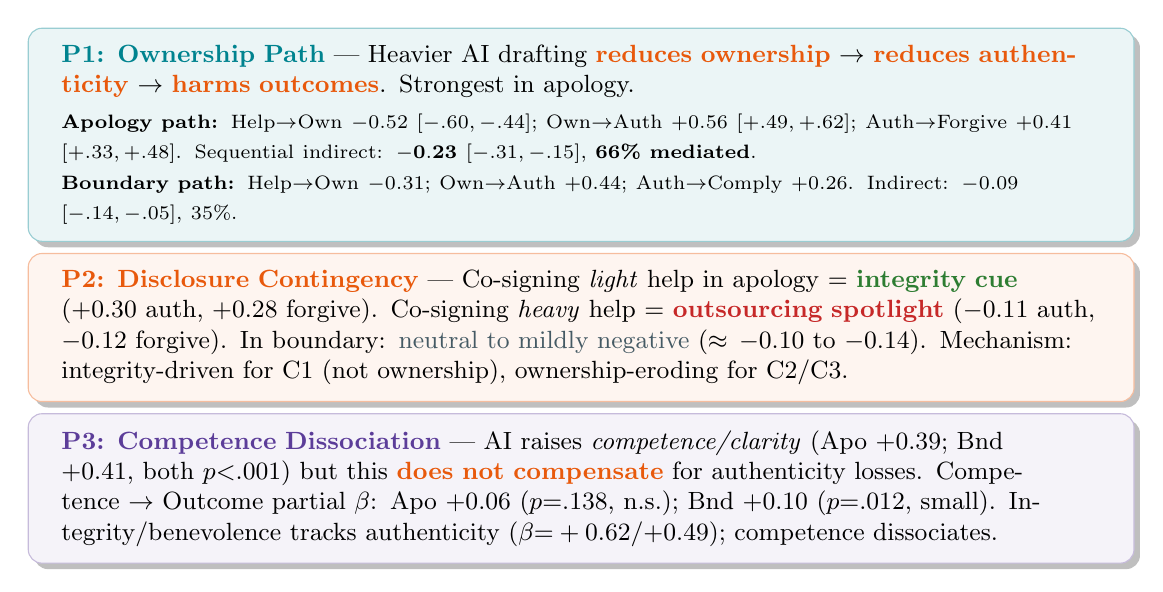
\begin{tikzpicture}[
  prop/.style={rounded corners=5pt, text width=13.2cm, align=left, font=\small,
    inner xsep=12pt, inner ysep=6pt,
    drop shadow}]

  \node[prop, fill=chiTeal!8, draw=chiTeal!40] (p1) at (0,0) {
    \textcolor{chiTeal}{\textbf{P1: Ownership Path}} --- Heavier AI drafting \emphmark{reduces ownership} $\to$ \emphmark{reduces authenticity}
    $\to$ \emphmark{harms outcomes}. Strongest in apology.\\[2pt]
    {\scriptsize \textbf{Apology path:} Help$\to$Own $-0.52$ [$-.60,-.44$]; Own$\to$Auth $+0.56$ [$+.49,+.62$]; Auth$\to$Forgive $+0.41$ [$+.33,+.48$]. Sequential indirect: $\mathbf{-0.23}$ [$-.31,-.15$], \textbf{66\% mediated}.}\\
    {\scriptsize \textbf{Boundary path:} Help$\to$Own $-0.31$; Own$\to$Auth $+0.44$; Auth$\to$Comply $+0.26$. Indirect: $-0.09$ [$-.14,-.05$], 35\%.}};

  \node[prop, fill=chiAccent!6, draw=chiAccent!40, below=4pt of p1] (p2) {
    \textcolor{chiAccent}{\textbf{P2: Disclosure Contingency}} --- Co-signing \emph{light} help in apology = \textcolor{chiGreen}{\textbf{integrity cue}} ($+0.30$ auth, $+0.28$ forgive). Co-signing \emph{heavy} help = \textcolor{chiRed}{\textbf{outsourcing spotlight}} ($-0.11$ auth, $-0.12$ forgive). In boundary: \textcolor{chiGray}{neutral to mildly negative} ($\approx -0.10$ to $-0.14$). Mechanism: integrity-driven for C1 (not ownership), ownership-eroding for C2/C3.};

  \node[prop, fill=chiPurple!6, draw=chiPurple!35, below=4pt of p2] (p3) {
    \textcolor{chiPurple}{\textbf{P3: Competence Dissociation}} --- AI raises \emph{competence/clarity} (Apo $+0.39$; Bnd $+0.41$, both $p{<}.001$) but this \emphmark{does not compensate} for authenticity losses. Competence $\to$ Outcome partial $\beta$: Apo $+0.06$ ($p{=}.138$, n.s.); Bnd $+0.10$ ($p{=}.012$, small). Integrity/benevolence tracks authenticity ($\beta{=}+0.62$/$+0.49$); competence dissociates.};
\end{tikzpicture}
\end{frame}

% ============================================================

\begin{frame}{Summary of Effects Across Scenarios}
\sideAccent
\vspace{2pt}
\scriptsize
\renewcommand{\arraystretch}{1.2}
\begin{center}
\begin{tabular}{@{}p{3.2cm} >{\centering\arraybackslash}p{5cm} >{\centering\arraybackslash}p{5cm}@{}}
  \toprule
  & \textbf{Apology / Repair} & \textbf{Boundary Request}\\
  \midrule
  Heavy help effect on ownership
    & \textcolor{chiRed}{\textbf{Strong negative}} ($-0.52$, CI $[-.60,-.44]$)
    & \textcolor{chiRed}{Moderate negative} ($-0.31$, CI $[-.38,-.24]$)\\[3pt]
  Co-sign + Tone
    & \textcolor{chiGreen}{\textbf{Positive}} ($d{=}0.28$, $p{<}.001$)
    & \textcolor{chiGray}{Neutral / mildly negative} ($d{=}{-}0.11$, $p{=}.051$)\\[3pt]
  Co-sign + Full
    & \textcolor{chiRed}{\textbf{Negative}} ($d{=}{-}0.10$, $p{=}.018$)
    & \textcolor{chiRed}{Mildly negative} ($d{=}{-}0.09$, $p{=}.088$)\\[3pt]
  Help penalty (C3)
    & $d{=}{-}0.76$ (Auth), $d{=}{-}0.54$ (Forgive)
    & $d{=}{-}0.35$ (Auth), $d{=}{-}0.18$ (Comply)\\[3pt]
  Competence/Clarity
    & Improved ($+0.39$, $p{<}.001$) but \textcolor{chiGray}{irrelevant} ($\beta{=}+0.06$, n.s.)
    & Improved ($+0.41$, $p{<}.001$), \textcolor{chiGray}{weakly helpful} ($\beta{=}+0.10$)\\[3pt]
  Mediation strength
    & \textbf{66\%} via ownership path
    & 35\% via ownership path\\[3pt]
  Sender miscalibration
    & Calibrated ($\Delta{\approx}0$)
    & \textcolor{chiAccent}{\textbf{Overestimates}} ($\Delta{=}+0.24$)\\
  \bottomrule
\end{tabular}
\end{center}
\end{frame}

% ============================================================

\begin{frame}{Five Design Principles for AI-Assisted Intimacy}
\sideAccent
\vspace{1pt}
\begin{tikzpicture}[
  dp/.style={rounded corners=4pt, text width=13cm, align=left, font=\scriptsize,
    inner xsep=10pt, inner ysep=5pt,
    drop shadow},
  icon/.style={font=\normalsize, minimum width=1.5em}]

  \node[dp, fill=chiTeal!7, draw=chiTeal!30] (d1) at (0,0) {
    \textcolor{chiTeal}{\faPen~~\textbf{1. Preserve Voice}} --- Default to suggestion-level edits;
    scaffold dyad-specific details (nicknames, shared memories); make human edits visible.\\
    {\scriptsize\textcolor{chiGray}{Evidence: each idiosyncrasy cue $\to$ $+0.18$ ownership, $+0.16$ authenticity ($p{<}.001$). Tone HCR $= 0.85$ vs.\ Full $= 0.59$.}}};

  \node[dp, fill=chiAccent!5, draw=chiAccent!30, below=2pt of d1] (d2) {
    \textcolor{chiAccent}{\faRedo~~\textbf{2. Restore Ownership}} --- When help is heavy, require an
    ``in-own-words'' revision pass; prompt for personal grounding before submission.\\
    {\scriptsize\textcolor{chiGray}{Evidence: Full ownership penalty $-0.52$ (Apo) drives 66\% of forgiveness loss. HCR and edit distance predict receiver judgments.}}};

  \node[dp, fill=chiGreen!5, draw=chiGreen!30, below=2pt of d2] (d3) {
    \textcolor{chiGreen!80!black}{\faComments~~\textbf{3. Disclosure as Interaction}} --- Sender-voiced
    rationales; context-appropriate framing (care/clarity for apologies); avoid generic system badges.\\
    {\scriptsize\textcolor{chiGray}{Evidence: same co-sign $\to$ opposite effects by help level ($d{=}+0.28$ vs.\ $d{=}{-}0.10$). CPM boundary rules are couple-specific.}}};

  \node[dp, fill=chiPurple!5, draw=chiPurple!25, below=2pt of d3] (d4) {
    \textcolor{chiPurple}{\faBalanceScale~~\textbf{4. Decompose Trust}} --- Show authors that competence
    gains rarely offset authenticity costs; preview trade-off during drafting.\\
    {\scriptsize\textcolor{chiGray}{Evidence: Competence $\to$ Outcome $\beta{=}+0.06$ (n.s.) in apology. Integrity tracks authenticity ($\beta{=}+0.62$).}}};

  \node[dp, fill=chiBlue!5, draw=chiBlue!25, below=2pt of d4] (d5) {
    \textcolor{chiBlue}{\faUniversalAccess~~\textbf{5. Context \& Fairness}} --- Ownership-restoring
    scaffolds for accessibility users; couple-level controls for disclosure norms; author-facing provenance (HCR indicators).\\
    {\scriptsize\textcolor{chiGray}{Evidence: miscalibration data show norms are unsettled; interface-level transparency can surface social interpretations.}}};
\end{tikzpicture}
\end{frame}

% ============================================================

\begin{frame}{Limitations}
\sideAccent
\vspace{4pt}
\begin{columns}[T]
\begin{column}{0.48\textwidth}
  \begin{alertbox}[\faExclamationTriangle~~ Boundary Conditions]
  \scriptsize
  \begin{itemize}\setlength\itemsep{4pt}
    \item[\faExclamationCircle] \textbf{Independent raters}, not actual partners --- normative judgments, not dyadic outcomes. Effects may differ within couples with shared history and negotiated rules.
    \item[\faExclamationCircle] \textbf{Single disclosure format} tested (sender-voiced, clarity-framed postscript). Design space includes placement, framing, authorship, specificity.
    \item[\faExclamationCircle] \textbf{English only}, Malaysia sample --- cultural norms for apology \& disclosure vary across societies and languages.
  \end{itemize}
  \end{alertbox}
\end{column}
\begin{column}{0.48\textwidth}
  \begin{alertbox}[\faArrowRight~~ Scope \& Next Steps]
  \scriptsize
  \begin{itemize}\setlength\itemsep{4pt}
    \item[\faExclamationCircle] \textbf{Two anchor scenarios} only (apology, boundary). Need to extend to affection, deeper transgressions, synchronous modalities (voice, video).
    \item[\faExclamationCircle] \textbf{Intentions, not behavior} --- participants reported willingness to forgive/comply, not consequential actions.
    \item[\faArrowRight] \textbf{Next step:} Dyadic field experiments pairing writers with actual partners, orthogonally varying disclosure design, observing consequential behavior across cultures.
  \end{itemize}
  \end{alertbox}
\end{column}
\end{columns}
\end{frame}

% ============================================================
%  CONCLUSION
% ============================================================

\begin{frame}{Contributions}
\sideAccent
\vspace{4pt}
\begin{tikzpicture}[
  ctr/.style={rounded corners=5pt, text width=6cm, minimum height=2.2cm,
    align=left, font=\small, inner xsep=10pt, inner ysep=8pt,
    drop shadow}]

  \node[ctr, fill=chiTeal!8, draw=chiTeal!40] (c1) at (0,1.5) {
    \textcolor{chiTeal}{\faFlask~~\textbf{C1: Causal Estimates}}\\[4pt]
    Scenario-aware effects of help level \& disclosure on ownership, authenticity, trust facets, and outcomes across $N{=}856$ (S1+S2) with crossed random effects for participants \& stimuli};

  \node[ctr, fill=chiAccent!6, draw=chiAccent!35] (c2) at (7.2,1.5) {
    \textcolor{chiAccent}{\faCogs~~\textbf{C2: Attributional Account}}\\[4pt]
    Empirically grounded mechanism: ownership is the proximal currency of authenticity. Competence--integrity dissociation explains why polish $\neq$ better outcomes};

  \node[ctr, fill=chiGreen!6, draw=chiGreen!35] (c3) at (0,-1.5) {
    \textcolor{chiGreen!80!black}{\faExchange*~~\textbf{C3: Miscalibration Evidence}}\\[4pt]
    First empirical sender--receiver comparison under realistic disclosure mixtures. Senders overestimate light-help benefits in boundary requests ($\Delta{=}+0.24$)};

  \node[ctr, fill=chiPurple!6, draw=chiPurple!30] (c4) at (7.2,-1.5) {
    \textcolor{chiPurple}{\faDraftingCompass~~\textbf{C4: Design Guidance}}\\[4pt]
    Five principles: voice-preserving defaults, ownership-restoring scaffolds, disclosure as interaction, trust decomposition, CPM-aligned couple controls};
\end{tikzpicture}
\end{frame}

% ============================================================

\begin{frame}{Take-Home Message}
\vspace{1pt}
\begin{center}
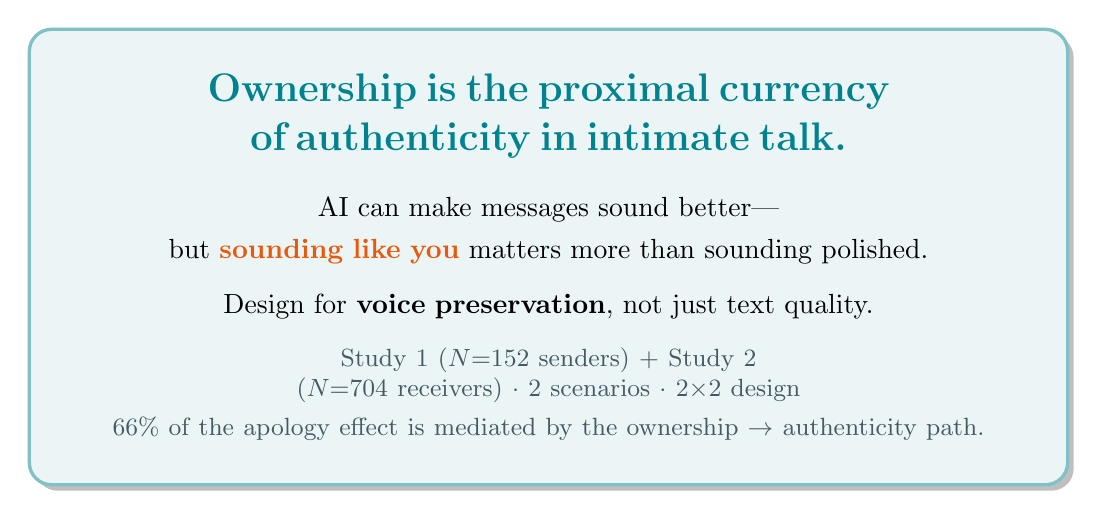
\begin{tikzpicture}
  \node[rounded corners=8pt, fill=chiTeal!8, draw=chiTeal!50, line width=1.2pt,
    inner xsep=24pt, inner ysep=16pt, text width=11.5cm, align=center,
    drop shadow] {
    {\Large\bfseries\textcolor{chiTeal}{Ownership is the proximal currency}}\\[4pt]
    {\Large\bfseries\textcolor{chiTeal}{of authenticity in intimate talk.}}\\[12pt]
    {\normalsize
    AI can make messages sound better---\\[3pt]
    but \emphmark{sounding like you} matters more than sounding polished.\\[8pt]
    Design for \textbf{voice preservation}, not just text quality.\\[8pt]
    {\small\textcolor{chiGray}{Study 1 ($N{=}152$ senders) + Study 2 ($N{=}704$ receivers) $\cdot$ 2 scenarios $\cdot$ 2$\times$2 design\\[2pt]
    66\% of the apology effect is mediated by the ownership $\to$ authenticity path.}}}
  };
\end{tikzpicture}
\end{center}

\vspace{1pt}
\begin{center}
{\small \textcolor{chiGray}{Guangrui Fan ~~\textbullet~~ fgr@tyust.edu.cn
 ~~\textbullet~~ DOI: \texttt{10.1145/3772318.3790762}}}
\end{center}
\end{frame}

% ============================================================
%  THANK YOU --- custom full-bleed
% ============================================================
{
\setbeamertemplate{footline}{}
\begin{frame}[plain,noframenumbering]
\begin{tikzpicture}[remember picture, overlay]
  % Background
  \fill[chiDeep] (current page.north west) rectangle (current page.south east);
  % Mosaic decorations
  \mosaicCorner{-6.5}{3.5}{2.0}
  \mosaicCorner{5.0}{3.0}{1.6}
  \mosaicCorner{-5.5}{-3.0}{1.4}
  \mosaicCorner{6.0}{-3.5}{1.8}

  % Thank you text
  \node[text=white, font=\Huge\bfseries] at ([yshift=12mm]current page.center)
    {Thank You!};
  \node[text=white!80, font=\large] at ([yshift=-2mm]current page.center)
    {Questions \& Discussion};

  % Contact info
  \node[text=white!70, font=\small, text width=10cm, align=center]
    at ([yshift=-18mm]current page.center) {
    \faEnvelope~~fgr@tyust.edu.cn \qquad
    \faFile*~~DOI: 10.1145/3772318.3790762};

  % Single white strip across bottom with all logos in one row
  \fill[white, opacity=0.92]
    ([yshift=0mm]current page.south west) rectangle
    ([yshift=16mm]current page.south east);
  \node[anchor=south west]
    at ([xshift=14mm, yshift=2mm]current page.south west)
    {
\includegraphics[height=1.1cm]{assets/tyust-logo.png}};
  \node[anchor=south]
    at ([xshift=-20mm, yshift=2.5mm]current page.south)
    {
\includegraphics[height=1.0cm]{assets/chi2026-logo.png}};
  \node[anchor=south]
    at ([xshift=20mm, yshift=2mm]current page.south)
    {
\includegraphics[height=1.0cm]{assets/acm-logo.png}};
  \node[anchor=south east]
    at ([xshift=-14mm, yshift=3mm]current page.south east)
    {
\includegraphics[height=0.9cm]{assets/sigchi-logo.png}};
\end{tikzpicture}
\end{frame}
}

% ============================================================
%  BACKUP / APPENDIX
% ============================================================
\appendix

\begin{frame}{Backup: Study 1 --- Model Fixed Effects}
\sideAccent
\vspace{4pt}
\small
\renewcommand{\arraystretch}{1.2}
\begin{center}
\begin{tabular}{@{}l ccc@{}}
  \toprule
  \textbf{Predictor} & \textbf{Ownership} & \textbf{Authenticity} & \textbf{Edit Dist.}\\
  \midrule
  Intercept & 5.10 $[4.92, 5.27]$ & 5.27 $[5.10, 5.45]$ & 0.18 $[0.16, 0.21]$\\
  Help (Full) & $-0.78$ $[-0.98,-0.58]$ & $-0.65$ $[-0.83,-0.47]$ & $+0.24$ $[0.20,0.28]$\\
  Scenario (Bnd) & $-0.32$ $[-0.47,-0.17]$ & $-0.41$ $[-0.55,-0.27]$ & $-0.03$ $[-0.06,0.00]$\\
  Help$\times$Scenario & $+0.14$ $[-0.06,0.34]$ & $-0.16$ $[-0.35,0.03]$ & $-0.05$ $[-0.09,-0.01]$\\
  \bottomrule
\end{tabular}
\end{center}
\vspace{2pt}
{\footnotesize\textcolor{chiGray}{All Help and Scenario main effects $p{<}.001$ except Edit Dist.\ Scenario ($p{=}.084$). Help$\times$Scenario significant for Edit Dist.\ ($p{=}.018$), n.s.\ otherwise. Participant random intercepts. Idiosyncrasy cues: Full $\to$ fewer (IRR $= 0.78$, CI $[0.71,0.86]$, $p{<}.001$); Boundary $\to$ fewer than Apology (IRR $= 0.68$, CI $[0.61,0.76]$, $p{<}.001$).}}
\end{frame}

% ============================================================

\begin{frame}{Backup: Study 2 --- Mediation Table}
\sideAccent
\vspace{4pt}
\small
\renewcommand{\arraystretch}{1.25}
\begin{center}
\begin{tabular}{@{}l cc@{}}
  \toprule
  \textbf{Contrast} & \textbf{Apology (indirect)} & \textbf{Boundary (indirect)}\\
  \midrule
  C1: Tone/CoSign $-$ Tone/None & $+0.01$ $[-0.01,+0.03]$ & $-0.03$ $[-0.06,-0.00]$\\
  C2: Full/CoSign $-$ Full/None & $-0.06$ $[-0.11,-0.02]$ & $-0.02$ $[-0.05,+0.01]$\\
  C3: Full/CoSign $-$ Tone/CoSign & $\mathbf{-0.23}$ $[-0.31,-0.15]$ & $\mathbf{-0.09}$ $[-0.14,-0.05]$\\
  \midrule
  \% Mediated (C3) & \textbf{66\%} & \textbf{35\%}\\
  \bottomrule
\end{tabular}
\end{center}
\vspace{2pt}
{\footnotesize\textcolor{chiGray}{Sequential indirect effects (standardized) via Effort/Ownership $\to$ Authenticity $\to$ Outcome. BCa 95\% CIs from 5{,}000 cluster bootstraps (participants \& stimuli). Bayesian multilevel mediation (brms) converged with frequentist estimates.}}
\end{frame}

% ============================================================

\begin{frame}{Backup: Stimulus-Level Predictors}
\sideAccent
\vspace{4pt}
\small
\renewcommand{\arraystretch}{1.25}
\begin{center}
\begin{tabular}{@{}l cc@{}}
  \toprule
  \textbf{S1 Predictor} & \textbf{S2 Effort/Ownership} & \textbf{S2 Authenticity}\\
  \midrule
  Idiosyncrasy cues (per cue) & $+0.18$ $[+0.12,+0.24]$, $p{<}.001$ & $+0.16$ $[+0.10,+0.22]$, $p{<}.001$\\
  Edit distance (0--1) & $-0.17$ $[-0.25,-0.09]$, $p{<}.001$ & $-0.12$ $[-0.19,-0.05]$, $p{=}.001$\\
  \midrule
  \multicolumn{3}{l}{\textit{By scenario (idiosyncrasy cues $\to$ Ownership):}}\\
  \quad Apology & $+0.21$ & \\
  \quad Boundary & $+0.14$ & \\
  \bottomrule
\end{tabular}
\end{center}
\vspace{2pt}
{\footnotesize\textcolor{chiGray}{Models include Help, Disclosure, Scenario, and Length as fixed effects; random intercepts for participant \& stimulus. Standardized coefficients. 40 unique messages as stimulus-level units.}}
\end{frame}

% ============================================================

\begin{frame}{Backup: Full Telemetry Details}
\sideAccent
\vspace{4pt}
\small
\renewcommand{\arraystretch}{1.1}
\begin{center}
\begin{tabular}{@{}l cccc@{}}
  \toprule
  & \multicolumn{2}{c}{\textbf{Apology}} & \multicolumn{2}{c}{\textbf{Boundary}}\\
  \cmidrule(lr){2-3}\cmidrule(lr){4-5}
  \textbf{Metric} & \textbf{Tone} & \textbf{Full} & \textbf{Tone} & \textbf{Full}\\
  \midrule
  Time-on-task (sec) & 341 (121) & 314 (136) & 327 (117) & 299 (128)\\
  Assistant calls & 2.1 (1.3) & 1.3 (0.6) & 1.7 (1.0) & 1.4 (0.7)\\
  Accept rate (Tone) & .62 (.21) & --- & .58 (.23) & ---\\
  Subst.\ edits (Full) & --- & 2.4 (1.5) & --- & 1.9 (1.3)\\
  Edit distance (0--1) & .19 (.10) & .44 (.14) & .17 (.09) & .39 (.13)\\
  HCR (0--1) & .86 (.08) & .60 (.12) & .84 (.09) & .58 (.11)\\
  Word count & 101 (14) & 99 (16) & 96 (15) & 95 (15)\\
  Idiosyncrasy cues & 1.9 (0.9) & 1.5 (0.8) & 1.3 (0.8) & 1.0 (0.7)\\
  \bottomrule
\end{tabular}
\end{center}
\vspace{2pt}
{\footnotesize\textcolor{chiGray}{Means (SD). GPT-4o via private API. Tone: temp $= 0.3$, content-adding blocked (9.7\% of proposed edits). Full: temp $= 0.2$, $\geq$1 substantive edit required.}}
\end{frame}

\end{document}
